% =====================================================================
%  Does Structural Change Predict Value?  Semantic information value as an
%  LLM-free admission signal for agent memory: a degeneracy analysis and a
%  matched-size test on LoCoMo and LongMemEval-S.
%  Build: cd paper2/paper && pdflatex main && bibtex main && pdflatex main && pdflatex main
%  Numbers: numbers.tex (python -m paper2.fill_numbers), numbers_lme.tex (python paper2/paper/make_numbers_lme.py) and numbers_online.tex
%  (python paper2/paper/make_numbers_online.py). No result is typed by hand.
%  Class: CEUR-ART if ceurart.cls is present (ESWC workshop), else LNCS
%  (llncs.cls, shipped here), else article.
% =====================================================================
\newif\ifceur
\newif\ifllncs
\IfFileExists{ceurart.cls}{\ceurtrue}{\IfFileExists{llncs.cls}{\llncstrue}{}}
\newif\ifanon \anonfalse % set \anontrue for the double-blind ESWC submission (removes name, affiliation, e-mail and repository URL)
\ifceur
  \documentclass{ceurart}
\else\ifllncs
  \documentclass[runningheads]{llncs}
\else
  \documentclass[11pt,a4paper]{article}
  \usepackage[margin=2.5cm]{geometry}
\fi\fi
\usepackage[utf8]{inputenc}
\usepackage[T1]{fontenc}
\usepackage{amsmath}
\usepackage{amssymb}
\usepackage{booktabs}
\usepackage{graphicx}
\usepackage{xcolor}
\usepackage{url}
\usepackage{array}
\usepackage{multirow}
\makeatletter
\@ifpackageloaded{hyperref}{}{\usepackage[hidelinks]{hyperref}}
\makeatother
\newif\ifshowtodos
\showtodostrue
\DeclareRobustCommand{\todo}[1]{\ifshowtodos{\color{red}\textbf{[TODO:} #1\textbf{]}}\fi}
% numbers.tex -- every quantitative result used by main.tex, as a macro.
% GENERATED FILE. The experiment code overwrites it; do not edit by hand.
% Default value for every macro is \todo{xx} so that an unfilled number is
% visible in the PDF. Keep every macro name; change only the values.
% Naming: <metric><Dataset><Policy>, <metric><Dataset><Category><Policy>,
% <hypothesis><quantity><Dataset>[<Category>]; see README.md for the contract.

% ---- Dataset and pipeline descriptives (filled by the code, not pre-registered constants)
\newcommand{\nCandTurnsLc}{2375}
\newcommand{\nCandTurnsLm}{\todo{xx}}
\newcommand{\nCandTriplesLc}{3199}
\newcommand{\nCandTriplesLm}{\todo{xx}}
\newcommand{\erPrecision}{\todo{xx}}
\newcommand{\erOracleHitGap}{\todo{xx}}
\newcommand{\gateAucCv}{\todo{xx}}
\newcommand{\gateNTrain}{\todo{xx}}
\newcommand{\gatePositives}{\todo{xx}}
\newcommand{\nTrainConvs}{\todo{xx}}

% ---- Degeneracy analysis of the 2010 measures and graph-shape preconditions (Section 6.1)
\newcommand{\fracSingleTriple}{0.718}
\newcommand{\nDistinctTedge}{10}
\newcommand{\fracTedgeZero}{0.773}
\newcommand{\fracTedgeOne}{0.061}
\newcommand{\hubImpactShare}{\todo{xx}}
\newcommand{\corrImpactSize}{0.001}
\newcommand{\corrSivaPlainSize}{-0.865}
\newcommand{\corrSivaPosition}{-0.854}
\newcommand{\corrSivaSivaPlain}{0.990}
\newcommand{\consFireRateLc}{0.000}
\newcommand{\consFireRateLm}{\todo{xx}}
\newcommand{\nonHubDegTwoShareLc}{0.133}
\newcommand{\nonHubEdgeShareLc}{0.000}
\newcommand{\nonHubDegTwoShareLm}{\todo{xx}}
\newcommand{\nonHubEdgeShareLm}{\todo{xx}}
\newcommand{\expansionFireRateLc}{\todo{xx}}

% ---- Main table, LoCoMo (Table main-locomo): hit / fone / admit / live / calls x policy
\newcommand{\hitLcAdmitAll}{0.643}
\newcommand{\foneLcAdmitAll}{\todo{xx}}
\newcommand{\admitLcAdmitAll}{1.00}
\newcommand{\liveLcAdmitAll}{2618}
\newcommand{\callsLcAdmitAll}{0}
\newcommand{\hitLcRandom}{0.379}
\newcommand{\foneLcRandom}{\todo{xx}}
\newcommand{\admitLcRandom}{0.48}
\newcommand{\liveLcRandom}{1315}
\newcommand{\callsLcRandom}{0}
\newcommand{\hitLcHeat}{0.405}
\newcommand{\foneLcHeat}{\todo{xx}}
\newcommand{\admitLcHeat}{0.46}
\newcommand{\liveLcHeat}{1309}
\newcommand{\callsLcHeat}{0}
\newcommand{\hitLcSivTen}{0.323}
\newcommand{\foneLcSivTen}{\todo{xx}}
\newcommand{\admitLcSivTen}{0.50}
\newcommand{\liveLcSivTen}{1301}
\newcommand{\callsLcSivTen}{0}
\newcommand{\hitLcGraphGate}{0.410}
\newcommand{\foneLcGraphGate}{\todo{xx}}
\newcommand{\admitLcGraphGate}{0.44}
\newcommand{\liveLcGraphGate}{1315}
\newcommand{\callsLcGraphGate}{0}
\newcommand{\hitLcAmacLite}{0.351}
\newcommand{\foneLcAmacLite}{\todo{xx}}
\newcommand{\admitLcAmacLite}{0.48}
\newcommand{\liveLcAmacLite}{1328}
\newcommand{\callsLcAmacLite}{0}
\newcommand{\hitLcAmac}{\todo{xx}}
\newcommand{\foneLcAmac}{\todo{xx}}
\newcommand{\admitLcAmac}{\todo{xx}}
\newcommand{\liveLcAmac}{\todo{xx}}
\newcommand{\callsLcAmac}{\todo{xx}}
\newcommand{\hitLcLlmGate}{\todo{xx}}
\newcommand{\foneLcLlmGate}{\todo{xx}}
\newcommand{\admitLcLlmGate}{\todo{xx}}
\newcommand{\liveLcLlmGate}{\todo{xx}}
\newcommand{\callsLcLlmGate}{\todo{xx}}
\newcommand{\hitLcLearned}{\todo{xx}}
\newcommand{\foneLcLearned}{\todo{xx}}
\newcommand{\admitLcLearned}{\todo{xx}}
\newcommand{\liveLcLearned}{\todo{xx}}
\newcommand{\callsLcLearned}{\todo{xx}}

% ---- Main table, LongMemEval-S (Table main-lme): hit / acc / admit / live / calls x policy
\newcommand{\hitLmAdmitAll}{\todo{xx}}
\newcommand{\accLmAdmitAll}{\todo{xx}}
\newcommand{\admitLmAdmitAll}{\todo{xx}}
\newcommand{\liveLmAdmitAll}{\todo{xx}}
\newcommand{\callsLmAdmitAll}{\todo{xx}}
\newcommand{\hitLmRandom}{\todo{xx}}
\newcommand{\accLmRandom}{\todo{xx}}
\newcommand{\admitLmRandom}{\todo{xx}}
\newcommand{\liveLmRandom}{\todo{xx}}
\newcommand{\callsLmRandom}{\todo{xx}}
\newcommand{\hitLmHeat}{\todo{xx}}
\newcommand{\accLmHeat}{\todo{xx}}
\newcommand{\admitLmHeat}{\todo{xx}}
\newcommand{\liveLmHeat}{\todo{xx}}
\newcommand{\callsLmHeat}{\todo{xx}}
\newcommand{\hitLmSivTen}{\todo{xx}}
\newcommand{\accLmSivTen}{\todo{xx}}
\newcommand{\admitLmSivTen}{\todo{xx}}
\newcommand{\liveLmSivTen}{\todo{xx}}
\newcommand{\callsLmSivTen}{\todo{xx}}
\newcommand{\hitLmGraphGate}{\todo{xx}}
\newcommand{\accLmGraphGate}{\todo{xx}}
\newcommand{\admitLmGraphGate}{\todo{xx}}
\newcommand{\liveLmGraphGate}{\todo{xx}}
\newcommand{\callsLmGraphGate}{\todo{xx}}
\newcommand{\hitLmAmacLite}{\todo{xx}}
\newcommand{\accLmAmacLite}{\todo{xx}}
\newcommand{\admitLmAmacLite}{\todo{xx}}
\newcommand{\liveLmAmacLite}{\todo{xx}}
\newcommand{\callsLmAmacLite}{\todo{xx}}
\newcommand{\hitLmAmac}{\todo{xx}}
\newcommand{\accLmAmac}{\todo{xx}}
\newcommand{\admitLmAmac}{\todo{xx}}
\newcommand{\liveLmAmac}{\todo{xx}}
\newcommand{\callsLmAmac}{\todo{xx}}
\newcommand{\hitLmLlmGate}{\todo{xx}}
\newcommand{\accLmLlmGate}{\todo{xx}}
\newcommand{\admitLmLlmGate}{\todo{xx}}
\newcommand{\liveLmLlmGate}{\todo{xx}}
\newcommand{\callsLmLlmGate}{\todo{xx}}
\newcommand{\hitLmLearned}{\todo{xx}}
\newcommand{\accLmLearned}{\todo{xx}}
\newcommand{\admitLmLearned}{\todo{xx}}
\newcommand{\liveLmLearned}{\todo{xx}}
\newcommand{\callsLmLearned}{\todo{xx}}

% ---- H1 contrast graph gate vs LLM gate
\newcommand{\hOneDiffLc}{\todo{xx}}
\newcommand{\hOneCiLc}{\todo{xx}}
\newcommand{\hOneSizeGapLc}{\todo{xx}}
\newcommand{\hOneDiffLm}{\todo{xx}}
\newcommand{\hOneCiLm}{\todo{xx}}
\newcommand{\hOneSizeGapLm}{\todo{xx}}
\newcommand{\seedSdAccLm}{\todo{xx}}
\newcommand{\seedSdHitLm}{\todo{xx}}
\newcommand{\seedSdFoneLc}{\todo{xx}}

% ---- Per-category table (Table percat)
\newcommand{\catLcSingleHopAdmitAll}{0.639}
\newcommand{\catLcSingleHopRandom}{0.353}
\newcommand{\catLcSingleHopGraphGate}{0.378}
\newcommand{\catLcSingleHopLlmGate}{\todo{xx}}
\newcommand{\catLcMultiHopAdmitAll}{0.633}
\newcommand{\catLcMultiHopRandom}{0.516}
\newcommand{\catLcMultiHopGraphGate}{0.523}
\newcommand{\catLcMultiHopLlmGate}{\todo{xx}}
\newcommand{\catLcTemporalAdmitAll}{0.722}
\newcommand{\catLcTemporalRandom}{0.394}
\newcommand{\catLcTemporalGraphGate}{0.431}
\newcommand{\catLcTemporalLlmGate}{\todo{xx}}
\newcommand{\catLcOpenDomainAdmitAll}{0.427}
\newcommand{\catLcOpenDomainRandom}{0.180}
\newcommand{\catLcOpenDomainGraphGate}{0.337}
\newcommand{\catLcOpenDomainLlmGate}{\todo{xx}}
\newcommand{\catLcAdversarialAdmitAll}{0.643}
\newcommand{\catLcAdversarialRandom}{0.370}
\newcommand{\catLcAdversarialGraphGate}{0.399}
\newcommand{\catLcAdversarialLlmGate}{\todo{xx}}
\newcommand{\catLmSsUserAdmitAll}{\todo{xx}}
\newcommand{\catLmSsUserRandom}{\todo{xx}}
\newcommand{\catLmSsUserGraphGate}{\todo{xx}}
\newcommand{\catLmSsUserLlmGate}{\todo{xx}}
\newcommand{\catLmSsAssistantAdmitAll}{\todo{xx}}
\newcommand{\catLmSsAssistantRandom}{\todo{xx}}
\newcommand{\catLmSsAssistantGraphGate}{\todo{xx}}
\newcommand{\catLmSsAssistantLlmGate}{\todo{xx}}
\newcommand{\catLmSsPreferenceAdmitAll}{\todo{xx}}
\newcommand{\catLmSsPreferenceRandom}{\todo{xx}}
\newcommand{\catLmSsPreferenceGraphGate}{\todo{xx}}
\newcommand{\catLmSsPreferenceLlmGate}{\todo{xx}}
\newcommand{\catLmMultiSessionAdmitAll}{\todo{xx}}
\newcommand{\catLmMultiSessionRandom}{\todo{xx}}
\newcommand{\catLmMultiSessionGraphGate}{\todo{xx}}
\newcommand{\catLmMultiSessionLlmGate}{\todo{xx}}
\newcommand{\catLmTemporalReasoningAdmitAll}{\todo{xx}}
\newcommand{\catLmTemporalReasoningRandom}{\todo{xx}}
\newcommand{\catLmTemporalReasoningGraphGate}{\todo{xx}}
\newcommand{\catLmTemporalReasoningLlmGate}{\todo{xx}}
\newcommand{\catLmKnowledgeUpdateAdmitAll}{\todo{xx}}
\newcommand{\catLmKnowledgeUpdateRandom}{\todo{xx}}
\newcommand{\catLmKnowledgeUpdateGraphGate}{\todo{xx}}
\newcommand{\catLmKnowledgeUpdateLlmGate}{\todo{xx}}

% ---- H2: SIVa vs value
\newcommand{\nPairsLc}{\todo{xx}}
\newcommand{\nPairsLm}{\todo{xx}}
\newcommand{\nAnswerCalls}{\todo{xx}}
\newcommand{\rhoLc}{\todo{xx}}
\newcommand{\rhoCiLc}{\todo{xx}}
\newcommand{\rhoLm}{\todo{xx}}
\newcommand{\rhoCiLm}{\todo{xx}}
\newcommand{\rhoPlainLc}{\todo{xx}}
\newcommand{\rhoPlainCiLc}{\todo{xx}}
\newcommand{\rhoPlainLm}{\todo{xx}}
\newcommand{\rhoPlainCiLm}{\todo{xx}}
\newcommand{\hTwoBetaLc}{\todo{xx}}
\newcommand{\hTwoBetaCiLc}{\todo{xx}}
\newcommand{\hTwoBetaLm}{\todo{xx}}
\newcommand{\hTwoBetaCiLm}{\todo{xx}}

% ---- H3: value per fact, all-new vs all-known vertices (Table h3)
\newcommand{\hThreeNewLcSingleHop}{\todo{xx}}
\newcommand{\hThreeKnownLcSingleHop}{\todo{xx}}
\newcommand{\hThreeDiffLcSingleHop}{\todo{xx}}
\newcommand{\hThreeCiLcSingleHop}{\todo{xx}}
\newcommand{\hThreeNLcSingleHop}{\todo{xx}}
\newcommand{\hThreeNewLcMultiHop}{\todo{xx}}
\newcommand{\hThreeKnownLcMultiHop}{\todo{xx}}
\newcommand{\hThreeDiffLcMultiHop}{\todo{xx}}
\newcommand{\hThreeCiLcMultiHop}{\todo{xx}}
\newcommand{\hThreeNLcMultiHop}{\todo{xx}}
\newcommand{\hThreeNewLcTemporal}{\todo{xx}}
\newcommand{\hThreeKnownLcTemporal}{\todo{xx}}
\newcommand{\hThreeDiffLcTemporal}{\todo{xx}}
\newcommand{\hThreeCiLcTemporal}{\todo{xx}}
\newcommand{\hThreeNLcTemporal}{\todo{xx}}
\newcommand{\hThreeNewLcOpenDomain}{\todo{xx}}
\newcommand{\hThreeKnownLcOpenDomain}{\todo{xx}}
\newcommand{\hThreeDiffLcOpenDomain}{\todo{xx}}
\newcommand{\hThreeCiLcOpenDomain}{\todo{xx}}
\newcommand{\hThreeNLcOpenDomain}{\todo{xx}}
\newcommand{\hThreeNewLcAdversarial}{\todo{xx}}
\newcommand{\hThreeKnownLcAdversarial}{\todo{xx}}
\newcommand{\hThreeDiffLcAdversarial}{\todo{xx}}
\newcommand{\hThreeCiLcAdversarial}{\todo{xx}}
\newcommand{\hThreeNLcAdversarial}{\todo{xx}}
\newcommand{\hThreeNewLmSsUser}{\todo{xx}}
\newcommand{\hThreeKnownLmSsUser}{\todo{xx}}
\newcommand{\hThreeDiffLmSsUser}{\todo{xx}}
\newcommand{\hThreeCiLmSsUser}{\todo{xx}}
\newcommand{\hThreeNLmSsUser}{\todo{xx}}
\newcommand{\hThreeNewLmSsAssistant}{\todo{xx}}
\newcommand{\hThreeKnownLmSsAssistant}{\todo{xx}}
\newcommand{\hThreeDiffLmSsAssistant}{\todo{xx}}
\newcommand{\hThreeCiLmSsAssistant}{\todo{xx}}
\newcommand{\hThreeNLmSsAssistant}{\todo{xx}}
\newcommand{\hThreeNewLmSsPreference}{\todo{xx}}
\newcommand{\hThreeKnownLmSsPreference}{\todo{xx}}
\newcommand{\hThreeDiffLmSsPreference}{\todo{xx}}
\newcommand{\hThreeCiLmSsPreference}{\todo{xx}}
\newcommand{\hThreeNLmSsPreference}{\todo{xx}}
\newcommand{\hThreeNewLmMultiSession}{\todo{xx}}
\newcommand{\hThreeKnownLmMultiSession}{\todo{xx}}
\newcommand{\hThreeDiffLmMultiSession}{\todo{xx}}
\newcommand{\hThreeCiLmMultiSession}{\todo{xx}}
\newcommand{\hThreeNLmMultiSession}{\todo{xx}}
\newcommand{\hThreeNewLmTemporalReasoning}{\todo{xx}}
\newcommand{\hThreeKnownLmTemporalReasoning}{\todo{xx}}
\newcommand{\hThreeDiffLmTemporalReasoning}{\todo{xx}}
\newcommand{\hThreeCiLmTemporalReasoning}{\todo{xx}}
\newcommand{\hThreeNLmTemporalReasoning}{\todo{xx}}
\newcommand{\hThreeNewLmKnowledgeUpdate}{\todo{xx}}
\newcommand{\hThreeKnownLmKnowledgeUpdate}{\todo{xx}}
\newcommand{\hThreeDiffLmKnowledgeUpdate}{\todo{xx}}
\newcommand{\hThreeCiLmKnowledgeUpdate}{\todo{xx}}
\newcommand{\hThreeNLmKnowledgeUpdate}{\todo{xx}}

% ---- H4: poisoning (Table poison)
\newcommand{\poisN}{1206}
\newcommand{\poisMarginalSrc}{\todo{xx}}
\newcommand{\poisMarginalTier}{\todo{xx}}
\newcommand{\poisQaBaseAdmitAll}{\todo{xx}}
\newcommand{\poisAdmitAdmitAllTwoSrc}{\todo{xx}}
\newcommand{\poisHarmAdmitAllTwoSrc}{\todo{xx}}
\newcommand{\poisAdmitAdmitAllTwoTier}{\todo{xx}}
\newcommand{\poisHarmAdmitAllTwoTier}{\todo{xx}}
\newcommand{\poisAdmitAdmitAllTenSrc}{\todo{xx}}
\newcommand{\poisHarmAdmitAllTenSrc}{\todo{xx}}
\newcommand{\poisAdmitAdmitAllTenTier}{\todo{xx}}
\newcommand{\poisHarmAdmitAllTenTier}{\todo{xx}}
\newcommand{\poisQaBaseSivTen}{\todo{xx}}
\newcommand{\poisAdmitSivTenTwoSrc}{\todo{xx}}
\newcommand{\poisHarmSivTenTwoSrc}{\todo{xx}}
\newcommand{\poisAdmitSivTenTwoTier}{\todo{xx}}
\newcommand{\poisHarmSivTenTwoTier}{\todo{xx}}
\newcommand{\poisAdmitSivTenTenSrc}{\todo{xx}}
\newcommand{\poisHarmSivTenTenSrc}{\todo{xx}}
\newcommand{\poisAdmitSivTenTenTier}{\todo{xx}}
\newcommand{\poisHarmSivTenTenTier}{\todo{xx}}
\newcommand{\poisQaBaseGraphGate}{\todo{xx}}
\newcommand{\poisAdmitGraphGateTwoSrc}{\todo{xx}}
\newcommand{\poisHarmGraphGateTwoSrc}{\todo{xx}}
\newcommand{\poisAdmitGraphGateTwoTier}{\todo{xx}}
\newcommand{\poisHarmGraphGateTwoTier}{\todo{xx}}
\newcommand{\poisAdmitGraphGateTenSrc}{0.322}
\newcommand{\poisHarmGraphGateTenSrc}{\todo{xx}}
\newcommand{\poisAdmitGraphGateTenTier}{0.104}
\newcommand{\poisHarmGraphGateTenTier}{\todo{xx}}
\newcommand{\poisQaBaseAmacLite}{\todo{xx}}
\newcommand{\poisAdmitAmacLiteTwoSrc}{\todo{xx}}
\newcommand{\poisHarmAmacLiteTwoSrc}{\todo{xx}}
\newcommand{\poisAdmitAmacLiteTwoTier}{\todo{xx}}
\newcommand{\poisHarmAmacLiteTwoTier}{\todo{xx}}
\newcommand{\poisAdmitAmacLiteTenSrc}{\todo{xx}}
\newcommand{\poisHarmAmacLiteTenSrc}{\todo{xx}}
\newcommand{\poisAdmitAmacLiteTenTier}{\todo{xx}}
\newcommand{\poisHarmAmacLiteTenTier}{\todo{xx}}
\newcommand{\poisQaBaseLlmGate}{\todo{xx}}
\newcommand{\poisAdmitLlmGateTwoSrc}{\todo{xx}}
\newcommand{\poisHarmLlmGateTwoSrc}{\todo{xx}}
\newcommand{\poisAdmitLlmGateTwoTier}{\todo{xx}}
\newcommand{\poisHarmLlmGateTwoTier}{\todo{xx}}
\newcommand{\poisAdmitLlmGateTenSrc}{\todo{xx}}
\newcommand{\poisHarmLlmGateTenSrc}{\todo{xx}}
\newcommand{\poisAdmitLlmGateTenTier}{\todo{xx}}
\newcommand{\poisHarmLlmGateTenTier}{\todo{xx}}

% ---- Ablation of the measures (Table ablation)
\newcommand{\ablAucSivTen}{0.431}
\newcommand{\ablHitSivTen}{\todo{xx}}
\newcommand{\ablFoneSivTen}{\todo{xx}}
\newcommand{\ablAucAnchor}{0.488}
\newcommand{\ablHitAnchor}{\todo{xx}}
\newcommand{\ablFoneAnchor}{\todo{xx}}
\newcommand{\ablAucSoft}{0.427}
\newcommand{\ablHitSoft}{\todo{xx}}
\newcommand{\ablFoneSoft}{\todo{xx}}
\newcommand{\ablAucLogImpact}{0.493}
\newcommand{\ablHitLogImpact}{\todo{xx}}
\newcommand{\ablFoneLogImpact}{\todo{xx}}
\newcommand{\ablAucNovelty}{0.518}
\newcommand{\ablHitNovelty}{\todo{xx}}
\newcommand{\ablFoneNovelty}{\todo{xx}}
\newcommand{\ablAucNoTier}{\todo{xx}}
\newcommand{\ablHitNoTier}{\todo{xx}}
\newcommand{\ablFoneNoTier}{\todo{xx}}
\newcommand{\ablAucFull}{\todo{xx}}
\newcommand{\ablHitFull}{\todo{xx}}
\newcommand{\ablFoneFull}{\todo{xx}}

% ---- Cost per 1,000 candidates
\newcommand{\callsPerKExtract}{\todo{xx}}
\newcommand{\tokensPerKExtract}{\todo{xx}}
\newcommand{\callsPerKLlmGate}{\todo{xx}}
\newcommand{\tokensPerKLlmGate}{\todo{xx}}
\newcommand{\callsPerKAmac}{\todo{xx}}
\newcommand{\tokensPerKAmac}{\todo{xx}}
\newcommand{\secondsPerKGraphGate}{\todo{xx}}

% 315 macros

% ---- Extra macros written by paper2.fill_numbers (policies the skeleton did not anticipate; wire into main.tex as needed)
\newcommand{\admitLcAmacFit}{0.48}
\newcommand{\admitLcGraphGateFull}{0.41}
\newcommand{\admitLcGraphGateStruct}{0.46}
\newcommand{\admitLcImpactTen}{0.49}
\newcommand{\callsLcAmacFit}{0}
\newcommand{\callsLcGraphGateFull}{0}
\newcommand{\callsLcGraphGateStruct}{0}
\newcommand{\callsLcImpactTen}{0}
\newcommand{\catLcAdversarialAmacFit}{0.350}
\newcommand{\catLcAdversarialAmacLite}{0.318}
\newcommand{\catLcAdversarialGraphGateFull}{0.408}
\newcommand{\catLcAdversarialGraphGateStruct}{0.422}
\newcommand{\catLcAdversarialHeat}{0.363}
\newcommand{\catLcAdversarialImpactTen}{0.332}
\newcommand{\catLcAdversarialSivTen}{0.296}
\newcommand{\catLcMultiHopAmacFit}{0.452}
\newcommand{\catLcMultiHopAmacLite}{0.470}
\newcommand{\catLcMultiHopGraphGateFull}{0.544}
\newcommand{\catLcMultiHopGraphGateStruct}{0.566}
\newcommand{\catLcMultiHopHeat}{0.495}
\newcommand{\catLcMultiHopImpactTen}{0.384}
\newcommand{\catLcMultiHopSivTen}{0.399}
\newcommand{\catLcOpenDomainAmacFit}{0.292}
\newcommand{\catLcOpenDomainAmacLite}{0.292}
\newcommand{\catLcOpenDomainGraphGateFull}{0.303}
\newcommand{\catLcOpenDomainGraphGateStruct}{0.303}
\newcommand{\catLcOpenDomainHeat}{0.292}
\newcommand{\catLcOpenDomainImpactTen}{0.258}
\newcommand{\catLcOpenDomainSivTen}{0.337}
\newcommand{\catLcSingleHopAmacFit}{0.360}
\newcommand{\catLcSingleHopAmacLite}{0.328}
\newcommand{\catLcSingleHopGraphGateFull}{0.384}
\newcommand{\catLcSingleHopGraphGateStruct}{0.398}
\newcommand{\catLcSingleHopHeat}{0.367}
\newcommand{\catLcSingleHopImpactTen}{0.334}
\newcommand{\catLcSingleHopSivTen}{0.300}
\newcommand{\catLcTemporalAmacFit}{0.422}
\newcommand{\catLcTemporalAmacLite}{0.369}
\newcommand{\catLcTemporalGraphGateFull}{0.553}
\newcommand{\catLcTemporalGraphGateStruct}{0.447}
\newcommand{\catLcTemporalHeat}{0.516}
\newcommand{\catLcTemporalImpactTen}{0.366}
\newcommand{\catLcTemporalSivTen}{0.353}
\newcommand{\hitCiHiLcAmacFit}{0.399}
\newcommand{\hitCiHiLcAmacLite}{0.372}
\newcommand{\hitCiHiLcGraphGate}{0.431}
\newcommand{\hitCiHiLcGraphGateFull}{0.457}
\newcommand{\hitCiHiLcGraphGateStruct}{0.453}
\newcommand{\hitCiHiLcHeat}{0.426}
\newcommand{\hitCiHiLcImpactTen}{0.364}
\newcommand{\hitCiHiLcRandom}{0.401}
\newcommand{\hitCiHiLcSivTen}{0.343}
\newcommand{\hitCiLoLcAmacFit}{0.356}
\newcommand{\hitCiLoLcAmacLite}{0.330}
\newcommand{\hitCiLoLcGraphGate}{0.389}
\newcommand{\hitCiLoLcGraphGateFull}{0.414}
\newcommand{\hitCiLoLcGraphGateStruct}{0.409}
\newcommand{\hitCiLoLcHeat}{0.383}
\newcommand{\hitCiLoLcImpactTen}{0.321}
\newcommand{\hitCiLoLcRandom}{0.358}
\newcommand{\hitCiLoLcSivTen}{0.303}
\newcommand{\hitLcAmacFit}{0.378}
\newcommand{\hitLcAmacFitAtQuarter}{0.224}
\newcommand{\hitLcAmacFitAtThreeQuarter}{0.521}
\newcommand{\hitLcAmacLiteAtQuarter}{0.205}
\newcommand{\hitLcAmacLiteAtThreeQuarter}{0.520}
\newcommand{\hitLcGraphGateAtQuarter}{0.229}
\newcommand{\hitLcGraphGateAtThreeQuarter}{0.548}
\newcommand{\hitLcGraphGateFull}{0.436}
\newcommand{\hitLcGraphGateFullAtQuarter}{0.262}
\newcommand{\hitLcGraphGateFullAtThreeQuarter}{0.578}
\newcommand{\hitLcGraphGateStruct}{0.431}
\newcommand{\hitLcGraphGateStructAtQuarter}{0.240}
\newcommand{\hitLcGraphGateStructAtThreeQuarter}{0.577}
\newcommand{\hitLcHeatAtQuarter}{0.196}
\newcommand{\hitLcHeatAtThreeQuarter}{0.562}
\newcommand{\hitLcImpactTen}{0.342}
\newcommand{\hitLcImpactTenAtQuarter}{0.128}
\newcommand{\hitLcImpactTenAtThreeQuarter}{0.459}
\newcommand{\hitLcRandomAtQuarter}{0.197}
\newcommand{\hitLcRandomAtThreeQuarter}{0.508}
\newcommand{\hitLcSivTenAtQuarter}{0.149}
\newcommand{\hitLcSivTenAtThreeQuarter}{0.470}
\newcommand{\liveLcAmacFit}{1304}
\newcommand{\liveLcGraphGateFull}{1301}
\newcommand{\liveLcGraphGateStruct}{1335}
\newcommand{\liveLcImpactTen}{1316}
\newcommand{\poisAdmitGraphGateStructTenSrc}{0.340}
\newcommand{\poisAdmitGraphGateStructTenTier}{0.097}
\newcommand{\poisAdmitRandomTenSrc}{0.288}
\newcommand{\poisAdmitRandomTenTier}{0.187}
\newcommand{\poisRetrievedShareGraphGateStructTenSrc}{0.996}
\newcommand{\poisRetrievedShareGraphGateStructTenTier}{0.950}
\newcommand{\poisRetrievedShareGraphGateTenSrc}{0.997}
\newcommand{\poisRetrievedShareGraphGateTenTier}{0.959}
\newcommand{\poisRetrievedShareRandomTenSrc}{0.997}
\newcommand{\poisRetrievedShareRandomTenTier}{0.990}
\newcommand{\sizeGapLcAmacFit}{0.017}
\newcommand{\sizeGapLcAmacLite}{0.027}
\newcommand{\sizeGapLcGraphGate}{0.018}
\newcommand{\sizeGapLcGraphGateFull}{0.019}
\newcommand{\sizeGapLcGraphGateStruct}{0.018}
\newcommand{\sizeGapLcHeat}{0.018}
\newcommand{\sizeGapLcImpactTen}{0.036}
\newcommand{\sizeGapLcRandom}{0.021}
\newcommand{\sizeGapLcSivTen}{0.030}

% generated by paper2/paper/make_numbers_online.py; do not edit
\newcommand{\foneOneAdmitAll}{0.427}
\newcommand{\emOneAdmitAll}{0.322}
\newcommand{\abstOneAdmitAll}{0.544}
\newcommand{\hitOneAdmitAll}{0.643}
\newcommand{\foneOneAdmitAllSingleHop}{0.390}
\newcommand{\hitOneAdmitAllSingleHop}{0.639}
\newcommand{\foneOneAdmitAllMultiHop}{0.242}
\newcommand{\hitOneAdmitAllMultiHop}{0.633}
\newcommand{\foneOneAdmitAllTemporal}{0.058}
\newcommand{\hitOneAdmitAllTemporal}{0.722}
\newcommand{\foneOneAdmitAllOpenDomain}{0.131}
\newcommand{\hitOneAdmitAllOpenDomain}{0.427}
\newcommand{\foneOneAdmitAllAdversarial}{0.942}
\newcommand{\hitOneAdmitAllAdversarial}{0.643}
\newcommand{\foneOneStruct}{0.369}
\newcommand{\emOneStruct}{0.298}
\newcommand{\abstOneStruct}{0.673}
\newcommand{\hitOneStruct}{0.431}
\newcommand{\foneOneStructSingleHop}{0.260}
\newcommand{\hitOneStructSingleHop}{0.398}
\newcommand{\foneOneStructMultiHop}{0.206}
\newcommand{\hitOneStructMultiHop}{0.566}
\newcommand{\foneOneStructTemporal}{0.037}
\newcommand{\hitOneStructTemporal}{0.447}
\newcommand{\foneOneStructOpenDomain}{0.100}
\newcommand{\hitOneStructOpenDomain}{0.303}
\newcommand{\foneOneStructAdversarial}{0.975}
\newcommand{\hitOneStructAdversarial}{0.422}
\newcommand{\foneOneRandom}{0.358}
\newcommand{\emOneRandom}{0.284}
\newcommand{\abstOneRandom}{0.679}
\newcommand{\hitOneRandom}{0.379}
\newcommand{\foneOneRandomSingleHop}{0.246}
\newcommand{\hitOneRandomSingleHop}{0.353}
\newcommand{\foneOneRandomMultiHop}{0.198}
\newcommand{\hitOneRandomMultiHop}{0.516}
\newcommand{\foneOneRandomTemporal}{0.034}
\newcommand{\hitOneRandomTemporal}{0.394}
\newcommand{\foneOneRandomOpenDomain}{0.088}
\newcommand{\hitOneRandomOpenDomain}{0.180}
\newcommand{\foneOneRandomAdversarial}{0.962}
\newcommand{\hitOneRandomAdversarial}{0.370}
\newcommand{\hitCondOneOne}{0.362}
\newcommand{\hitCondZeroOne}{0.082}
\newcommand{\hitCondDiffOne}{+0.280}
\newcommand{\hitCondNoneOne}{2232}
\newcommand{\hitCondNzeroOne}{2361}
\newcommand{\rhoDhitDfoneOne}{+0.52}
\newcommand{\signAgreeOne}{7}
\newcommand{\dFoneStructRandomOne}{+0.013}
\newcommand{\pFoneStructRandomOne}{0.105}
\newcommand{\winsFoneStructRandomOne}{6}
\newcommand{\ciFoneStructRandomLoOne}{-0.003}
\newcommand{\ciFoneStructRandomHiOne}{+0.029}
\newcommand{\hitCondDiffOneSingleHop}{+0.430}
\newcommand{\hitCondDiffOneMultiHop}{+0.172}
\newcommand{\hitCondDiffOneTemporal}{+0.074}
\newcommand{\hitCondDiffOneOpenDomain}{+0.053}
\newcommand{\foneTwoAdmitAll}{0.491}
\newcommand{\emTwoAdmitAll}{0.343}
\newcommand{\abstTwoAdmitAll}{0.469}
\newcommand{\hitTwoAdmitAll}{0.643}
\newcommand{\foneTwoAdmitAllSingleHop}{0.440}
\newcommand{\hitTwoAdmitAllSingleHop}{0.639}
\newcommand{\foneTwoAdmitAllMultiHop}{0.242}
\newcommand{\hitTwoAdmitAllMultiHop}{0.633}
\newcommand{\foneTwoAdmitAllTemporal}{0.318}
\newcommand{\hitTwoAdmitAllTemporal}{0.722}
\newcommand{\foneTwoAdmitAllOpenDomain}{0.148}
\newcommand{\hitTwoAdmitAllOpenDomain}{0.427}
\newcommand{\foneTwoAdmitAllAdversarial}{0.944}
\newcommand{\hitTwoAdmitAllAdversarial}{0.643}
\newcommand{\foneTwoStruct}{0.408}
\newcommand{\emTwoStruct}{0.304}
\newcommand{\abstTwoStruct}{0.617}
\newcommand{\hitTwoStruct}{0.431}
\newcommand{\foneTwoStructSingleHop}{0.284}
\newcommand{\hitTwoStructSingleHop}{0.398}
\newcommand{\foneTwoStructMultiHop}{0.206}
\newcommand{\hitTwoStructMultiHop}{0.566}
\newcommand{\foneTwoStructTemporal}{0.212}
\newcommand{\hitTwoStructTemporal}{0.447}
\newcommand{\foneTwoStructOpenDomain}{0.133}
\newcommand{\hitTwoStructOpenDomain}{0.303}
\newcommand{\foneTwoStructAdversarial}{0.969}
\newcommand{\hitTwoStructAdversarial}{0.422}
\newcommand{\foneTwoRandom}{0.388}
\newcommand{\emTwoRandom}{0.290}
\newcommand{\abstTwoRandom}{0.622}
\newcommand{\hitTwoRandom}{0.379}
\newcommand{\foneTwoRandomSingleHop}{0.266}
\newcommand{\hitTwoRandomSingleHop}{0.353}
\newcommand{\foneTwoRandomMultiHop}{0.186}
\newcommand{\hitTwoRandomMultiHop}{0.516}
\newcommand{\foneTwoRandomTemporal}{0.183}
\newcommand{\hitTwoRandomTemporal}{0.394}
\newcommand{\foneTwoRandomOpenDomain}{0.088}
\newcommand{\hitTwoRandomOpenDomain}{0.180}
\newcommand{\foneTwoRandomAdversarial}{0.957}
\newcommand{\hitTwoRandomAdversarial}{0.370}
\newcommand{\hitCondOneTwo}{0.461}
\newcommand{\hitCondZeroTwo}{0.101}
\newcommand{\hitCondDiffTwo}{+0.360}
\newcommand{\hitCondNoneTwo}{2232}
\newcommand{\hitCondNzeroTwo}{2361}
\newcommand{\rhoDhitDfoneTwo}{+0.92}
\newcommand{\signAgreeTwo}{7}
\newcommand{\dFoneStructRandomTwo}{+0.026}
\newcommand{\pFoneStructRandomTwo}{0.064}
\newcommand{\winsFoneStructRandomTwo}{6}
\newcommand{\ciFoneStructRandomLoTwo}{-0.002}
\newcommand{\ciFoneStructRandomHiTwo}{+0.054}
\newcommand{\hitCondDiffTwoSingleHop}{+0.474}
\newcommand{\hitCondDiffTwoMultiHop}{+0.180}
\newcommand{\hitCondDiffTwoTemporal}{+0.306}
\newcommand{\hitCondDiffTwoOpenDomain}{+0.106}
\newcommand{\memzNconv}{10}
\newcommand{\memzAdmitRate}{0.975}
\newcommand{\memzAdmitRateMin}{0.921}
\newcommand{\memzAdmitRateMax}{0.989}
\newcommand{\memzLive}{2582}
\newcommand{\memzCalls}{2375}
\newcommand{\memzParseFail}{3}
\newcommand{\memzAdd}{2434}
\newcommand{\memzUpdate}{75}
\newcommand{\memzDelete}{0}
\newcommand{\memzNone}{11344}
\newcommand{\memzCallsPerK}{742}
\newcommand{\memzTokensPerK}{2,074,667}
\newcommand{\memzFracOfAdmitAll}{0.986}
\newcommand{\memzHit}{0.638}
\newcommand{\hitMemz}{0.638}
\newcommand{\foneMemz}{0.488}
\newcommand{\liveMemz}{2582}
\newcommand{\hitStructAtMemz}{0.640}
\newcommand{\foneStructAtMemz}{0.490}
\newcommand{\liveStructAtMemz}{2501}
\newcommand{\hitRandomAtMemz}{0.623}
\newcommand{\foneRandomAtMemz}{0.481}
\newcommand{\liveRandomAtMemz}{2484}
\newcommand{\hOneDiffFone}{+0.11}
\newcommand{\hOneCiLo}{-1.02}
\newcommand{\hOneCiHi}{+1.24}
\newcommand{\hOneDiffHit}{+0.003}
\newcommand{\extHandCheckOk}{8}
\newcommand{\extHandCheckWeak}{4}
\newcommand{\extHandCheckWrong}{6}
\newcommand{\extHandCheckN}{18}
\newcommand{\extFallbackShare}{2.9\%}
\newcommand{\extFunctionalTriples}{8}
\newcommand{\extInvalidations}{0}
\newcommand{\obsSpeakerSubjShare}{84.6\%}
\newcommand{\obsPossSubjShare}{6.0\%}
\newcommand{\obsNonSpeakerSubjShare}{2.3\%}
\newcommand{\obsParseFailShare}{6.5\%}
\newcommand{\rawTurnsTwoNE}{1.0\%}
\newcommand{\rawTurnsOneNE}{11.8\%}
\newcommand{\lmeTurnsTwoNE}{15.5\%}
\newcommand{\lmeTurnsOneNE}{41.2\%}
\newcommand{\ruleCedgesMin}{4}
\newcommand{\ruleCedgesMax}{64}
\newcommand{\ruleBedgesMax}{6}
\newcommand{\nObsSentences}{2{,}541}
\newcommand{\permRandomMean}{+0.057}
\newcommand{\permRandomCiLo}{+0.030}
\newcommand{\permRandomCiHi}{+0.085}
\newcommand{\permRandomP}{0.004}
\newcommand{\permRandomHolm}{0.023}
\newcommand{\permRandomWins}{9}
\newcommand{\permSivTenMean}{+0.112}
\newcommand{\permSivTenCiLo}{+0.052}
\newcommand{\permSivTenCiHi}{+0.172}
\newcommand{\permSivTenP}{0.002}
\newcommand{\permSivTenHolm}{0.016}
\newcommand{\permSivTenWins}{10}
\newcommand{\permImpactTenMean}{+0.089}
\newcommand{\permImpactTenCiLo}{+0.050}
\newcommand{\permImpactTenCiHi}{+0.128}
\newcommand{\permImpactTenP}{0.002}
\newcommand{\permImpactTenHolm}{0.016}
\newcommand{\permImpactTenWins}{10}
\newcommand{\permHeatMean}{+0.027}
\newcommand{\permHeatCiLo}{-0.000}
\newcommand{\permHeatCiHi}{+0.054}
\newcommand{\permHeatP}{0.049}
\newcommand{\permHeatHolm}{0.146}
\newcommand{\permHeatWins}{8}
\newcommand{\permAmacLiteMean}{+0.081}
\newcommand{\permAmacLiteCiLo}{+0.040}
\newcommand{\permAmacLiteCiHi}{+0.123}
\newcommand{\permAmacLiteP}{0.006}
\newcommand{\permAmacLiteHolm}{0.029}
\newcommand{\permAmacLiteWins}{9}
\newcommand{\permAmacFitMean}{+0.057}
\newcommand{\permAmacFitCiLo}{+0.018}
\newcommand{\permAmacFitCiHi}{+0.096}
\newcommand{\permAmacFitP}{0.008}
\newcommand{\permAmacFitHolm}{0.031}
\newcommand{\permAmacFitWins}{8}
\newcommand{\permGraphGateMean}{+0.022}
\newcommand{\permGraphGateCiLo}{-0.002}
\newcommand{\permGraphGateCiHi}{+0.046}
\newcommand{\permGraphGateP}{0.074}
\newcommand{\permGraphGateHolm}{0.148}
\newcommand{\permGraphGateWins}{7}
\newcommand{\permGraphGateFullMean}{-0.004}
\newcommand{\permGraphGateFullCiLo}{-0.033}
\newcommand{\permGraphGateFullCiHi}{+0.026}
\newcommand{\permGraphGateFullP}{0.861}
\newcommand{\permGraphGateFullHolm}{0.861}
\newcommand{\permGraphGateFullWins}{6}
\newcommand{\hThreeNewSingleHop}{0.258}
\newcommand{\hThreeKnownSingleHop}{0.215}
\newcommand{\hThreeDiffSingleHop}{+0.044}
\newcommand{\hThreeNewCiSingleHop}{[0.238, 0.279]}
\newcommand{\hThreeKnownCiSingleHop}{[0.179, 0.255]}
\newcommand{\hThreeNnewSingleHop}{1724}
\newcommand{\hThreeNknownSingleHop}{438}
\newcommand{\hThreeNewMultiHop}{0.244}
\newcommand{\hThreeKnownMultiHop}{0.185}
\newcommand{\hThreeDiffMultiHop}{+0.059}
\newcommand{\hThreeNewCiMultiHop}{[0.225, 0.265]}
\newcommand{\hThreeKnownCiMultiHop}{[0.151, 0.224]}
\newcommand{\hThreeNnewMultiHop}{1724}
\newcommand{\hThreeNknownMultiHop}{438}
\newcommand{\hThreeNewTemporal}{0.116}
\newcommand{\hThreeKnownTemporal}{0.094}
\newcommand{\hThreeDiffTemporal}{+0.022}
\newcommand{\hThreeNewCiTemporal}{[0.102, 0.132]}
\newcommand{\hThreeKnownCiTemporal}{[0.070, 0.125]}
\newcommand{\hThreeNnewTemporal}{1724}
\newcommand{\hThreeNknownTemporal}{438}
\newcommand{\hThreeNewOpenDomain}{0.061}
\newcommand{\hThreeKnownOpenDomain}{0.037}
\newcommand{\hThreeDiffOpenDomain}{+0.025}
\newcommand{\hThreeNewCiOpenDomain}{[0.051, 0.074]}
\newcommand{\hThreeKnownCiOpenDomain}{[0.023, 0.059]}
\newcommand{\hThreeNnewOpenDomain}{1724}
\newcommand{\hThreeNknownOpenDomain}{438}
\newcommand{\hThreeNewAdversarial}{0.148}
\newcommand{\hThreeKnownAdversarial}{0.112}
\newcommand{\hThreeDiffAdversarial}{+0.037}
\newcommand{\hThreeNewCiAdversarial}{[0.132, 0.166]}
\newcommand{\hThreeKnownCiAdversarial}{[0.086, 0.145]}
\newcommand{\hThreeNnewAdversarial}{1724}
\newcommand{\hThreeNknownAdversarial}{438}
\newcommand{\hThreeNewAll}{0.470}
\newcommand{\hThreeKnownAll}{0.390}
\newcommand{\hThreeDiffAll}{+0.080}
\newcommand{\hThreeNewCiAll}{[0.447, 0.494]}
\newcommand{\hThreeKnownCiAll}{[0.346, 0.437]}
\newcommand{\hThreeNnewAll}{1724}
\newcommand{\hThreeNknownAll}{438}
\newcommand{\haikuCalls}{21,156}
\newcommand{\haikuInTokens}{24.0}
\newcommand{\haikuOutTokens}{1.13}
\newcommand{\haikuCostUsd}{2.97}

% generated by paper2/paper/make_numbers_lme.py; do not edit
\newcommand{\lmeCiHiHitFitHeat}{+0.203}
\newcommand{\lmeCiHiHitFitPrior}{+0.105}
\newcommand{\lmeCiHiHitFitRandom}{+0.119}
\newcommand{\lmeCiHiHitPriorRandom}{+0.056}
\newcommand{\lmeCiHiHitRandomHeat}{+0.127}
\newcommand{\lmeCiHiMrrFitHeat}{+0.161}
\newcommand{\lmeCiHiMrrFitPrior}{+0.077}
\newcommand{\lmeCiHiMrrFitRandom}{+0.117}
\newcommand{\lmeCiHiMrrPriorRandom}{+0.077}
\newcommand{\lmeCiHiMrrRandomHeat}{+0.075}
\newcommand{\lmeCiLoHitFitHeat}{+0.106}
\newcommand{\lmeCiLoHitFitPrior}{+0.024}
\newcommand{\lmeCiLoHitFitRandom}{+0.027}
\newcommand{\lmeCiLoHitPriorRandom}{-0.040}
\newcommand{\lmeCiLoHitRandomHeat}{+0.036}
\newcommand{\lmeCiLoMrrFitHeat}{+0.077}
\newcommand{\lmeCiLoMrrFitPrior}{+0.008}
\newcommand{\lmeCiLoMrrFitRandom}{+0.043}
\newcommand{\lmeCiLoMrrPriorRandom}{-0.001}
\newcommand{\lmeCiLoMrrRandomHeat}{+0.003}
\newcommand{\lmeCvAucMax}{0.706}
\newcommand{\lmeCvAucMin}{0.689}
\newcommand{\lmeDHitFitHeat}{+0.154}
\newcommand{\lmeDHitFitPrior}{+0.065}
\newcommand{\lmeDHitFitRandom}{+0.073}
\newcommand{\lmeDHitPriorRandom}{+0.008}
\newcommand{\lmeDHitRandomHeat}{+0.081}
\newcommand{\lmeDMrrFitHeat}{+0.119}
\newcommand{\lmeDMrrFitPrior}{+0.043}
\newcommand{\lmeDMrrFitRandom}{+0.080}
\newcommand{\lmeDMrrPriorRandom}{+0.038}
\newcommand{\lmeDMrrRandomHeat}{+0.039}
\newcommand{\lmeFracAdmitAll}{0.411}
\newcommand{\lmeFracFit}{0.262}
\newcommand{\lmeFracHeat}{0.143}
\newcommand{\lmeFracPrior}{0.212}
\newcommand{\lmeFracRandom}{0.202}
\newcommand{\lmeHitAdmitAll}{0.574}
\newcommand{\lmeHitAdmitAllKnowledgeUpdate}{0.694}
\newcommand{\lmeHitAdmitAllMultiSession}{0.728}
\newcommand{\lmeHitAdmitAllSsAssistant}{0.143}
\newcommand{\lmeHitAdmitAllSsPreference}{0.533}
\newcommand{\lmeHitAdmitAllSsUser}{0.562}
\newcommand{\lmeHitAdmitAllTemporalReasoning}{0.561}
\newcommand{\lmeHitFit}{0.399}
\newcommand{\lmeHitFitKnowledgeUpdate}{0.486}
\newcommand{\lmeHitFitMultiSession}{0.576}
\newcommand{\lmeHitFitSsAssistant}{0.071}
\newcommand{\lmeHitFitSsPreference}{0.300}
\newcommand{\lmeHitFitSsUser}{0.266}
\newcommand{\lmeHitFitTemporalReasoning}{0.409}
\newcommand{\lmeHitHeat}{0.244}
\newcommand{\lmeHitHeatKnowledgeUpdate}{0.278}
\newcommand{\lmeHitHeatMultiSession}{0.312}
\newcommand{\lmeHitHeatSsAssistant}{0.107}
\newcommand{\lmeHitHeatSsPreference}{0.167}
\newcommand{\lmeHitHeatSsUser}{0.125}
\newcommand{\lmeHitHeatTemporalReasoning}{0.295}
\newcommand{\lmeHitPrior}{0.334}
\newcommand{\lmeHitPriorKnowledgeUpdate}{0.333}
\newcommand{\lmeHitPriorMultiSession}{0.448}
\newcommand{\lmeHitPriorSsAssistant}{0.054}
\newcommand{\lmeHitPriorSsPreference}{0.333}
\newcommand{\lmeHitPriorSsUser}{0.328}
\newcommand{\lmeHitPriorTemporalReasoning}{0.348}
\newcommand{\lmeHitRandom}{0.326}
\newcommand{\lmeHitRandomKnowledgeUpdate}{0.361}
\newcommand{\lmeHitRandomMultiSession}{0.440}
\newcommand{\lmeHitRandomSsAssistant}{0.107}
\newcommand{\lmeHitRandomSsPreference}{0.300}
\newcommand{\lmeHitRandomSsUser}{0.250}
\newcommand{\lmeHitRandomTemporalReasoning}{0.333}
\newcommand{\lmeHolmHitFitHeat}{0.000}
\newcommand{\lmeHolmHitFitPrior}{0.006}
\newcommand{\lmeHolmHitFitRandom}{0.006}
\newcommand{\lmeKHitFitHeat}{479}
\newcommand{\lmeKHitFitPrior}{479}
\newcommand{\lmeKHitFitRandom}{479}
\newcommand{\lmeKHitPriorRandom}{479}
\newcommand{\lmeKHitRandomHeat}{479}
\newcommand{\lmeKMrrFitHeat}{479}
\newcommand{\lmeKMrrFitPrior}{479}
\newcommand{\lmeKMrrFitRandom}{479}
\newcommand{\lmeKMrrPriorRandom}{479}
\newcommand{\lmeKMrrRandomHeat}{479}
\newcommand{\lmeLiveAdmitAll}{167,482}
\newcommand{\lmeLiveFit}{84,038}
\newcommand{\lmeLiveHeat}{83,786}
\newcommand{\lmeLivePrior}{83,679}
\newcommand{\lmeLiveRandom}{83,784}
\newcommand{\lmeLossesHitFitHeat}{39}
\newcommand{\lmeLossesHitFitPrior}{34}
\newcommand{\lmeLossesHitFitRandom}{46}
\newcommand{\lmeLossesHitPriorRandom}{66}
\newcommand{\lmeLossesHitRandomHeat}{43}
\newcommand{\lmeLossesMrrFitHeat}{60}
\newcommand{\lmeLossesMrrFitPrior}{58}
\newcommand{\lmeLossesMrrFitRandom}{63}
\newcommand{\lmeLossesMrrPriorRandom}{80}
\newcommand{\lmeLossesMrrRandomHeat}{59}
\newcommand{\lmeMrrAdmitAll}{0.362}
\newcommand{\lmeMrrFit}{0.291}
\newcommand{\lmeMrrHeat}{0.172}
\newcommand{\lmeMrrPrior}{0.249}
\newcommand{\lmeMrrRandom}{0.211}
\newcommand{\lmeNq}{500}
\newcommand{\lmePHitFitHeat}{0.000}
\newcommand{\lmePHitFitPrior}{0.003}
\newcommand{\lmePHitFitRandom}{0.003}
\newcommand{\lmePHitPriorRandom}{0.798}
\newcommand{\lmePHitRandomHeat}{0.001}
\newcommand{\lmePMrrFitHeat}{0.000}
\newcommand{\lmePMrrFitPrior}{0.015}
\newcommand{\lmePMrrFitRandom}{0.000}
\newcommand{\lmePMrrPriorRandom}{0.057}
\newcommand{\lmePMrrRandomHeat}{0.033}
\newcommand{\lmeWImpactMax}{+1.11}
\newcommand{\lmeWImpactMin}{+0.99}
\newcommand{\lmeWNoveltyMax}{+0.40}
\newcommand{\lmeWNoveltyMin}{+0.31}
\newcommand{\lmeWinsHitFitHeat}{113}
\newcommand{\lmeWinsHitFitPrior}{65}
\newcommand{\lmeWinsHitFitRandom}{81}
\newcommand{\lmeWinsHitPriorRandom}{70}
\newcommand{\lmeWinsHitRandomHeat}{82}
\newcommand{\lmeWinsMrrFitHeat}{133}
\newcommand{\lmeWinsMrrFitPrior}{90}
\newcommand{\lmeWinsMrrFitRandom}{113}
\newcommand{\lmeWinsMrrPriorRandom}{96}
\newcommand{\lmeWinsMrrRandomHeat}{97}

\setlength{\emergencystretch}{3em}
\setlength{\tabcolsep}{4pt}
\renewcommand{\topfraction}{0.85}
\renewcommand{\textfraction}{0.1}
\renewcommand{\floatpagefraction}{0.7}
\newcommand{\Gc}{G_c}
\newcommand{\Gt}{G_t}
\newcommand{\Gcp}{G_c'}
\newcommand{\Ec}{E_c}
\newcommand{\Et}{E_t}
\newcommand{\Ecp}{E_c'}
\newcommand{\Vc}{V_c}
\newcommand{\Vt}{V_t}
\newcommand{\Hub}{H}
\newcommand{\Tedge}{T_{\mathrm{edge}}}
\newcommand{\Tsoft}{T_{\mathrm{soft}}}
\newcommand{\Anc}{A}
\newcommand{\Imp}{I}
\newcommand{\Implog}{I'}
\newcommand{\Nov}{N}
\newcommand{\Novp}{N_p}
\newcommand{\SIVp}{\mathrm{SIV}_p}
\newcommand{\SIVa}{\mathrm{SIV}_a}
\newcommand{\SIVaplain}{\mathrm{SIV}_a^{\mathrm{plain}}}
\newcommand{\degv}{\deg}
\newcommand{\cons}{c}
\newcommand{\code}[1]{\texttt{#1}}
\newcommand{\papertitle}{Does Structural Change Predict Value? Semantic Information Value as an LLM-Free Admission Signal for Agent Memory: A Degeneracy Analysis and a Matched-Size Test on LoCoMo and LongMemEval-S}
\newcommand{\shorttitle}{Does Structural Change Predict Value?}

\newcommand{\theabstract}{%
Agent memory systems decide what to store with a language-model call per candidate fact. We ask whether the structure of the memory graph carries that information, and give the first implementation and quantitative test, in an agent-memory setting, of al-Saffar and Heileman's 2010 semantic information value (SIV): trust times degree-weighted impact, and the realised graph-edit change of a write. At fact granularity the formulation is degenerate: on LoCoMo trust is exactly zero for a share \fracTedgeZero{} of candidates, the product ranks below random admission at every memory budget, and the realised change is a clock (Spearman \corrSivaPosition{} with position) because consolidation never fires. A redesign that separates anchoring from agreement, excludes speaker hubs from impact and adds pattern novelty, fitted leave-one-conversation-out and compared at matched memory size, retains more gold evidence than random (\permRandomMean{} evidence hit, exact permutation $p=\permRandomP$), than the 2010 measures and than A-MAC's lexical features, but no more than a turn-length heuristic. On LongMemEval-S (\lmeNq{} independent memories) the same gate, cross-fitted over questions, retains \lmeDHitFitRandom{} more evidence than random ($p=\lmePHitFitRandom$) while the turn-length heuristic falls below random. Answering the questions with a fixed model confirms that the offline proxy carries signal but overstates the gate's benefit (F1 gain over random \dFoneStructRandomTwo{}, $p=\pFoneStructRandomTwo$). Mem0's verbatim gate admits \memzAdmitRate{} of candidate turns at \memzCallsPerK{} model calls per thousand, so it does not gate here. Under sourceless poisoning the gate admits more false facts than random; provenance weighting is the defence. Pre-registration, code, run artefacts and number files are released.%
}

\begin{document}
\ifceur
  \copyrightyear{2027}
  \copyrightclause{Copyright for this paper by its authors. Use permitted under Creative Commons License Attribution 4.0 International (CC BY 4.0).}
  \conference{Workshop at ESWC 2027 (to be confirmed), Limassol, Cyprus, 23--27 May 2027}
  \title{\papertitle}
  \author[1]{Mohammad Zuber Taj}[email=us.zubertaj@gmail.com]
  \address[1]{Independent researcher, New Jersey, United States}
  \begin{abstract}\theabstract\end{abstract}
  \begin{keywords}agent memory \sep knowledge graphs \sep information value \sep admission control \sep provenance \sep pre-registration\end{keywords}
  \maketitle
\else
  \ifllncs
    \title{\papertitle}
    \titlerunning{\shorttitle}
    \author{Mohammad Zuber Taj\inst{1}}
    \authorrunning{Taj}
        \ifanon
      \author{Anonymous author}
      \authorrunning{Anonymous}
      \institute{Anonymous institution}
    \else
      \author{Mohammad Zuber Taj\inst{1}}
      \authorrunning{M.~Z. Taj}
      \institute{Independent researcher, New Jersey, United States\\ \email{us.zubertaj@gmail.com}}
    \fi
    \maketitle
    \begin{abstract}\theabstract
      \keywords{agent memory \and knowledge graphs \and information value \and admission control \and provenance \and pre-registration}
    \end{abstract}
  \else
    \title{\papertitle}
    \author{Mohammad Zuber Taj\\ Independent researcher}
    \date{Draft of \today}
    \maketitle
    \begin{abstract}\theabstract\end{abstract}
  \fi
\fi

% =====================================================================
\section{Introduction}
\label{sec:intro}

Long-term memory for conversational agents is a write path with a gate: a candidate fact is extracted from a turn and a decision is made to add it, to update or invalidate what it contradicts, or to drop it. In most systems that report results on the public long-conversation benchmarks, that decision is a language-model call. Mem0 asks a model to choose among \textsc{add}, \textsc{update}, \textsc{delete} and \textsc{none} (\textsc{noop} in the paper's wording)~\cite{chhikara2025mem0}; Zep's Graphiti resolves duplicates and invalidates contradicted edges with model prompts~\cite{rasmussen2025zep,graphiti}; Nemori spends two calls per write on a predicted schema and its deviation~\cite{nemori2025}; GAM defines a graph divergence as its consolidation trigger and then declines to compute it, calling the computation ``expensive and sensitive to lexical noise'', and uses a model as a proxy~\cite{gam2026}. The cheap alternatives are usage-based (MemoryOS promotes by a heat score of visits, length and recency~\cite{kang2025memoryos}) or text-based (A-MAC scores confidence by ROUGE-L and novelty by embedding distance, with one model call for utility~\cite{zhang2026amac}). None of them scores a candidate by the structure of the memory graph it lands in.

That structure was proposed as a value signal before there were agents to use it. In 2008 al-Saffar and Heileman introduced the recipient's world-view graph (their 2010 paper names it the \emph{context graph}) and valued a piece of information by the impact it would have on it and the trust in its source~\cite{alsaffar2008impact,alsaffar2008valuation}; in 2010 they cast both as RDF graph properties~\cite{alsaffar2010siv}: \emph{trust} as the share of the target's edges already in the context graph, \emph{impact} as the degree-weighted share of overlapping vertices, their product as the \emph{predicted} semantic information value, and the edit distance, with uniform costs, between the context graph before and after learning as the \emph{actual} value. The measures are linear-time because IRI labels make vertex alignment trivial. They were demonstrated in a browser plug-in over DBpedia and never evaluated quantitatively; the authors wrote that traditional evaluation does not apply to subjective valuation. We found no later implementation (the first author's publication page lists only PDFs) and no agent-memory paper that cites them.

\paragraph{Claim under test.} Graph-structural features of a candidate memory fact (agreement with what the memory holds, anchoring to known entities, degree-weighted impact, pattern novelty) carry measurable information about the fact's downstream value for question answering, at zero gate-time model calls.

\paragraph{What this paper is not.} It does not propose a new measure. Trust, impact and the two SIVs are al-Saffar and Heileman's; the novelty term is Joslyn and al-Saffar's motif information gain over the extant ontology~\cite{joslyn2011motifs,alsaffar2011extant}; agreement-based trust is Knowledge-Based Trust~\cite{dong2015kbt}; graph priors for fact admission are Knowledge Vault's~\cite{dong2014kv}; informativeness of triples is RELIN's~\cite{cheng2011relin}; the RDF delta is Berners-Lee and Connolly's~\cite{bernerslee2001delta}. What no work we could find does, as of the pre-registration date, is to admit agent-memory facts with a graph-informational measure and measure the result against question answering at matched memory size.

\paragraph{What we found, in one paragraph.} The 2010 measures degenerate at fact granularity, measurably and for arithmetic reasons (Section~\ref{sec:degeneracy}). A redesigned, LLM-free gate over seven graph features beats random, the 2010 measures and A-MAC's lexical features at matched memory size on LoCoMo but only matches a turn-length heuristic (Section~\ref{sec:matched}); on LongMemEval-S, cross-fitted over questions, it beats random while the length heuristic falls below random (Section~\ref{sec:lme}); answering the questions with a fixed model shows that the offline evidence-recall proxy carries signal but overstates the gate's benefit by about half (Section~\ref{sec:online}). The verbatim Mem0 gate admits nearly every candidate on LoCoMo, which turns the pre-registered non-inferiority question into a cost question (Section~\ref{sec:h1}); structural novelty admits poison unless provenance is weighted (Section~\ref{sec:h4}); and the memory graph has no entity-to-entity edges on either dataset, which on LoCoMo we trace to the benchmark's observations rather than to the extractor (Section~\ref{sec:shape}). The realised-change hypothesis (H2) is not tested on either arm as run and is deferred with the reasons stated.

\paragraph{Contributions.}
\begin{itemize}
  \item The first implementation and quantitative evaluation of SIV (trust, impact, $\SIVp$, $\SIVa$) in an agent-memory setting, under a pre-registered design, with a degeneracy analysis of the 2010 formulation at fact granularity and a redesign that separates agreement from anchoring and excludes hubs from impact (Sections~\ref{sec:measures} and~\ref{sec:degeneracy}).
  \item A matched-size, leave-one-conversation-out comparison protocol with an exact sign-flip permutation test over conversations, applied to nine LLM-free policies besides admit-all and to the verbatim Mem0 gate (Sections~\ref{sec:design}, \ref{sec:matched} and~\ref{sec:h1}).
  \item A validation of evidence recall, the offline proxy that every LLM-free development loop of this kind relies on, against answers from a fixed model, including the two pipeline details (dates on facts, the official temporal hint) without which temporal questions cannot be answered from a fact store (Section~\ref{sec:online}).
  \item A measurement of how reallocatable an agreement-and-novelty admission value is under self-consistent sourceless poisoning and how much a provenance tier recovers (Section~\ref{sec:h4}), complementary to Fei et al.~\cite{fei2026selection}.
  \item A graph-shape precondition table and a measurement showing that entity-to-entity topology is absent from LoCoMo's observations themselves (\obsNonSpeakerSubjShare{} non-speaker subjects), with the implication for where such claims can be tested (Section~\ref{sec:shape}).
  \item An offline replication of the matched-size test on LongMemEval-S with the question as the unit of inference, a gate cross-fitted per dataset, and the length-plus-revisit heuristic falling below random (Section~\ref{sec:lme}).
  \item Code, the frozen pre-registration with its deviation log, run artefacts and the number files behind every table.
\end{itemize}

% =====================================================================
\section{Background and related work}
\label{sec:related}

\subsection{Information value of graphs}
al-Saffar and Heileman introduced subjective information valuation in two 2008 papers~\cite{alsaffar2008impact,alsaffar2008valuation}: the value of an information piece to a consumer is a function of the impact it would have on a graph representing the consumer's world view (named the \emph{context graph} in the 2010 paper) and of the trust the consumer places in its provenance. Their 2010 paper~\cite{alsaffar2010siv} restates this over plain RDF graphs. Given a target graph $\Gt$ and a context graph $\Gc$, the \emph{actual} value is the dissimilarity between $\Gc$ and the revised graph $\Gcp=l(\Gc,\Gt)$ after learning (their eqs.~1--5), computed as a graph edit distance~\cite{bunke1997ged} with uniform costs, $(|\Ecp|-|\Ec|)/|\Ecp|$; the \emph{predicted} value replaces the unknown learning function by plain union (eq.~6) and non-uniform edge costs $t\times\degv(v)$ for edges attached to vertices the two graphs share, with cost 1 for the edges of new disconnected components (eq.~7); trust is the share of target edges already in the context (eq.~8), impact the degree-weighted share of shared vertices (eq.~9), and $\SIVp$ their product (eq.~10). The 2008 papers took trust from explicitly stated provenance; the 2010 paper derives it from agreement. Both framings matter here: our provenance tier is a return to the 2008 design, and our poisoning arm tests the 2010 one. al-Saffar, Joslyn and colleagues' \emph{extant ontology}, the frequency-weighted class--predicate--class graph computed by one aggregate query over a triple store~\cite{alsaffar2011extant}, and the information gain of typed motifs relative to independence~\cite{joslyn2011motifs} are the source of our novelty term. The delta of two RDF graphs as insert and delete sets, and the observation that blank nodes make it a graph-isomorphism problem while IRIs make it trivial, is older still~\cite{bernerslee2001delta}; our $\SIVa$ is a weighted instance of that delta.

Valuing triples by graph statistics has a decade of Semantic Web precedent that the agent-memory literature has not used: RELIN's informativeness from triple frequencies~\cite{cheng2011relin}, the entity-summarisation lineage that followed~\cite{liu2021entitysumm}, and the statistical rejection of implausible triples from predicate--type distributions~\cite{paulheim2014sdvalidate}. At web scale, Knowledge Vault fuses graph-based priors with extractor confidences and admits triples above a calibrated probability~\cite{dong2014kv}, and Knowledge-Based Trust estimates a source's trustworthiness from the correctness of the facts extracted from it~\cite{dong2015kbt}. The 2010 trust ratio is the naive version of that idea and lacks the extraction-error model; we return to this in Section~\ref{sec:threats}.

\subsection{Agent memory systems and their write paths}
We group the systems by what happens when a candidate fact arrives. \emph{LLM gates.} Mem0 extracts candidate memories and lets a model choose \textsc{add}, \textsc{update}, \textsc{delete} or \textsc{none} against the most similar stored memories (ten in the paper, five per candidate fact in the code)~\cite{chhikara2025mem0}; the open-source release carries this gate through tag 1.0.11 (the last PyPI release with it, April 2026); it is absent from tag 1.1.0 onwards, and the current code (2.2.1) writes through an add-only path, which is why we run the 1.0.11 prompt verbatim (Section~\ref{sec:policies}). Zep's Graphiti deduplicates entities and edges by model judgement after embedding and full-text candidate retrieval, invalidates contradicted edges by model judgement and keeps bitemporal validity~\cite{rasmussen2025zep,graphiti}. Nemori frames writing as prediction error but implements it as two model calls~\cite{nemori2025}. A-MEM lets a model write note attributes and links~\cite{xu2025amem}; Generative Agents score importance with a model at write time~\cite{park2023generative}; MemGPT makes the model manage its own memory tiers~\cite{packer2023memgpt}. \emph{Arithmetic gates.} MemoryOS promotes from mid- to long-term memory when a heat score (visits, interaction length, exponential recency) crosses a threshold~\cite{kang2025memoryos}; MemoryBank forgets by an Ebbinghaus curve~\cite{zhong2024memorybank}. \emph{LLM-light linear gates.} A-MAC scores a candidate by five factors (utility from one model call, ROUGE-L confidence, embedding novelty, recency, a type prior) with cross-validated weights; it reports admission-label precision and recall and no downstream QA, so we re-implement lexical analogues of its LLM-free features inside our pipeline (Table~\ref{tab:policies}), with novelty computed against the live memory (A-MAC's released experiment scripts compute it against an empty list) and recency omitted as constant at write time~\cite{zhang2026amac}. \emph{Learned gates.} Memory-R1 trains the manager with reinforcement learning; it remains a model call at inference~\cite{yan2025memoryr1}. \emph{Efficiency.} LightMem reports large reductions in calls and tokens through lightweight filtering~\cite{fang2025lightmem}; we therefore report write-path calls and tokens per thousand candidates rather than a headline fraction. \emph{Graph consolidation.} GAM declines to compute the graph divergence that would trigger consolidation~\cite{gam2026}; Kumiho lists degree-based entrenchment as future work~\cite{park2026kumiho}; HippoRAG's node specificity is a frequency-based graph weight applied at read time~\cite{gutierrez2024hipporag}; the 2026 systems that use degree or centrality (Selective Forgetting, EngramRAG and STRATA; arXiv 2608.28978, 2609.32049 and 2610.19386) apply it to prune or decay nodes or to protect them at garbage collection, after admission, and none scores a candidate before it is written. The surveys we consulted list no structural write policy~\cite{survey2025rethinking,survey2025memoryage}, and the 2026 survey of graph-based personalised memory (arXiv 2609.08599) names no system that uses degree, centrality or connectivity for write decisions; CoALA supplies the vocabulary~\cite{sumers2024coala}.

\subsection{Context graphs, selection integrity and benchmarks}
``Context graph'' now names a vendor category~\cite{garg2025contextgraphs} and a formal object with relation contexts~\cite{xu2024contextgraph}; al-Saffar and Heileman's sense predates both and, in their 2010 paper, came with a formula, and the memory graph of Section~\ref{sec:model} is a context graph in that sense. Fei et al.\ show that sourceless structural writes reroute the selector of a graph memory and silently misdirect downstream actions; exposure is predicted by the \emph{reallocatability} of the selector's structural term~\cite{fei2026selection,gutierrez2025hipporag2}. We infer, and Section~\ref{sec:h4} tests, that agreement-based trust, degree-based impact and pattern novelty, all computed over a writable memory graph, are reallocatable in their sense (Fei et al.\ do not discuss overlap-based trust, so the inference is ours), which makes the poisoning arm central rather than optional. LoCoMo~\cite{maharana2024locomo} releases ten long dyadic conversations with per-session observations, dialogue-turn evidence ids and five question categories; LongMemEval~\cite{wu2025longmemeval} releases 500 questions over per-question session haystacks with answer-bearing turns marked and a knowledge-update type. This paper uses LoCoMo for the full arm and LongMemEval-S for the offline matched-size replication (Section~\ref{sec:lme}); Section~\ref{sec:shape} explains why the deferred hypotheses need LongMemEval-S's entity density and knowledge-update questions.

% =====================================================================
\section{Problem statement and memory model}
\label{sec:model}

\paragraph{Setting.} A conversation arrives as a stream of turns grouped into sessions. A fixed extractor turns each turn into a candidate set $\Gt=(\Vt,\Et)$ of one to five typed triples $(s,p,o)$ with a source turn, a session, a speaker, an observation time, a provenance tier and a confidence. An \emph{admission policy} assigns the candidate a score; a \emph{gate} turns the score into an admit or reject decision; admitted triples are written into the memory graph $\Gc=(\Vc,\Ec)$; at the end of each session a consolidation step $\cons$ runs. Every question is then answered from a retrieval over the admitted graph that is identical for every policy. The only thing that varies between runs is the policy.

\paragraph{Memory model.} The memory is an entity-centric knowledge graph~\cite{hogan2021kg}. Nodes are entities typed Person, Place, Org, Event, Date, Pet, Thing or NamedEntity. Edges are facts $(s,p,o)$ with properties \code{source\_turns}, \code{session}, \code{speaker}, \code{observed\_at}, \code{tier} $\in$ \{verbatim-user, extractor-inferred, llm-summary, poisoned\}, \code{confidence}, \code{method}, \code{text}, \code{valid\_from} and \code{valid\_to}. Consolidation sets \code{valid\_to}; nothing is deleted, and ``live'' means \code{valid\_to} unset. The hub set $\Hub$ holds the two speakers; the measures exclude it where stated. Entity resolution applies four rules in order: exact match of the normalised surface form within type (R1), a hub-name match regardless of type (R2), Person/NamedEntity cross-type exact match (R3), and a token-sort fuzzy ratio of at least 90 within type for names of five or more characters with a length difference of at most twelve (R4)~\cite{bachmann2021rapidfuzz}; dates are never fuzzy-matched. The graph exports to RDF in reifier style~\cite{w3c2026rdf12}, under which the measures below are three aggregate queries.

\paragraph{Admission as score plus gate.} Every policy returns one score per candidate set and never sees gold evidence. Exact duplicates of live facts are suppressed for every policy, including admit-all. Two gates are used: a fixed threshold, and an \emph{online quantile} gate that admits a candidate when its score exceeds the running $(1-q)$ quantile of the scores seen so far in the conversation, decides the first $w=20$ warm-up candidates by alternation towards the target rate (identically for every policy), admits ties only while the realised rate is below $q$, nudges the quantile level by the gap between $q$ and the realised rate, and admits or rejects unconditionally while the realised rate is outside $q\pm0.05$ (a budget band added after the first runs, because a score that trends with graph size defeats any running quantile). Memory size is matched across policies by bisection on $q$ (Section~\ref{sec:design}, \emph{Matched size}).

% =====================================================================
\section{Measures}
\label{sec:measures}

All measures are LLM-free and linear in $|\Et|$ given degree, pattern and predicate counts maintained over the live edges. Let $\Gc=(\Vc,\Ec)$ be the live memory after entity resolution of the candidate's vertices, $\Gt=(\Vt,\Et)$ the candidate and $\Hub$ the hub set. Table~\ref{tab:measures} summarises the 2010 forms, why each degenerates at fact granularity, and the redesign.

\begin{table}[tp]
  \centering
  \caption{The 2010 measures, why each degenerates for one-to-five-triple candidates, and the redesign. The 2010 forms are kept and reported as policies.}
  \label{tab:measures}
  \small
  \begin{tabular}{@{}p{0.24\linewidth}p{0.38\linewidth}p{0.32\linewidth}@{}}
    \toprule
    2010 form & Why it degenerates here & Redesign \\
    \midrule
    Trust $\Tedge=|\Et\cap\Ec|/|\Et|$ & For $|\Et|\le 5$ it takes at most eleven values (\nDistinctTedge{} observed); a new fact scores 0, an exact duplicate scores 1, so trust $\times$ impact ranks redundancy above news. & Anchoring $\Anc$ (share of non-hub candidate vertices already known) and soft agreement $\Tsoft$ (best per-subject similarity): ``about known things'' versus ``already known''. \\
    \addlinespace
    Impact $\Imp=\frac{\sum_{v\in\Vt\cap\Vc}\degv v}{\sum_{v\in\Vc}\degv v}$ & The speakers sit in almost every triple and carry most of the degree mass. & $\Implog$: log-degree mass of shared \emph{non-hub} vertices over the same for memory. \\
    \addlinespace
    $\SIVp=\Tedge\times\Imp$ & Inherits both; zero for almost every non-duplicate. & Logistic gate over the features of Table~\ref{tab:features}, fitted leave-one-conversation-out. \\
    \addlinespace
    $\SIVa$ with $\Gcp=\Gc\cup\Gt$ (eq.~6) & Under plain union the delta is the new-triple ratio: content-blind and monotone in memory size. & $\Gcp=\cons(\Gc\cup\Gt)$ with a consolidation $\cons$ (entity merge, functional-fact invalidation, symmetric closure); the plain form is kept as a control. \\
    \addlinespace
    Directional prior: new disconnected knowledge costs 1, connected knowledge $t\times\degv v$ & Encodes ``new unknown concepts matter less'', which is backwards when gold evidence is new. & Tested as H3 rather than assumed. \\
    \bottomrule
  \end{tabular}
\end{table}

\paragraph{Trust, anchoring, soft agreement.} The 2010 trust is $\Tedge(\Gt,\Gc)=|\Et\cap\Ec|/|\Et|$, membership tested after entity resolution of $s$ and $o$ and exact match of $p$; it is reported as-is. The redesign separates two things the ratio conflates. \emph{Anchoring} is the share of non-hub candidate vertices already known,
\begin{equation}
  \Anc(\Gt,\Gc)=\frac{|(\Vt\setminus\Hub)\cap\Vc|}{|\Vt\setminus\Hub|},
  \label{eq:anchoring}
\end{equation}
undefined, and the candidate excluded from anchoring-based analyses, when $\Vt\setminus\Hub$ is empty. \emph{Soft agreement} is the mean, over candidate edges whose subject resolves, of the best token-set Jaccard similarity of the verbalised $(p,o)$ to a live fact with the same subject; unresolved subjects contribute zero.

\paragraph{Impact.} The 2010 impact $\Imp=\sum_{v\in\Vt\cap\Vc}\degv(v)/\sum_{v\in\Vc}\degv(v)$ is reported as-is. The redesign excludes hubs and damps degree: $\Implog=\sum_{v\in(\Vt\cap\Vc)\setminus\Hub}\log(1+\degv v)\,/\sum_{v\in\Vc\setminus\Hub}\log(1+\degv v)$. The pre-registered per-type variant was not implemented (Table~\ref{tab:deviations2}).

\paragraph{Novelty.} With $\Pi$ the set of patterns $(\tau(s),p,\tau(o))$ over live edges and $c(\pi)$ their counts, $\Nov(\Gt)=\frac{1}{|\Et|}\sum_{(s,p,o)\in\Et}-\log\hat p(\tau(s),p,\tau(o))$ with $\hat p(\pi)=(c(\pi)+1)/(|\Ec|+|\Pi|+1)$, and $\Novp$ is the same over predicates alone: the extant-ontology statistic of~\cite{alsaffar2011extant} used as a surprisal.

\paragraph{Predicted value.} $\SIVp=\Tedge\times\Imp$ is run unmodified as \code{siv\_2010}, and $\Imp$ alone as \code{impact\_2010}. The redesigned predicted value is a logistic function of the standardised feature vector of Table~\ref{tab:features}, with $\ell_2$-regularised, class-balanced weights fitted on the nine conversations other than the one evaluated on LoCoMo (Section~\ref{sec:matched-design}) and by five-fold cross-fitting over questions on LongMemEval-S (Section~\ref{sec:lme}). The label of a candidate is whether its source turn is a gold evidence turn of some question of the same conversation. Two fitted variants are run: the \emph{structural-only} gate over the seven graph features $\{\Tedge,\Anc,\Tsoft,\Imp,\Implog,\Nov,\Novp\}$, which is the headline policy, and the \emph{structural\,+\,surface} gate over all thirteen. A hand-set prior weight vector, fixed before any fitting but absent from the frozen pre-registration, is kept as a third, unfitted variant (\code{graph\_gate}); on raw features it is a novelty-minus-redundancy score.

\begin{table}[tp]
  \centering
  \caption{The feature vector of the gate (\code{measures.FEATURE\_NAMES}). The first seven rows are the graph-structural subset used by the headline policy. AUC is the area under the ROC curve of the single feature against the admission label over the \nCandTurnsLc{} candidate turns of the admit-all stream (Section~\ref{sec:degeneracy}).}
  \label{tab:features}
  \small
  \begin{tabular}{@{}llp{0.36\linewidth}r@{}}
    \toprule
    Code name & Symbol & Definition & AUC \\
    \midrule
    \code{t\_edge} & $\Tedge$ & the 2010 trust & 0.436 \\
    \code{anchoring} & $\Anc$ & eq.~\eqref{eq:anchoring} & \ablAucAnchor \\
    \code{t\_soft} & $\Tsoft$ & best per-subject Jaccard to a live fact & \ablAucSoft \\
    \code{impact} & $\Imp$ & the 2010 impact & 0.410 \\
    \code{impact\_log} & $\Implog$ & hub-excluded log-degree impact & \ablAucLogImpact \\
    \code{novelty} & $\Nov$ & pattern surprisal & \ablAucNovelty \\
    \code{novelty\_pred} & $\Novp$ & predicate surprisal & 0.507 \\
    \midrule
    \code{n\_edges} & $|\Et|$ & candidate size & 0.490 \\
    \code{n\_new\_vertices} & -- & non-hub candidate vertices not in $\Vc$ & 0.575 \\
    \code{n\_nonhub} & $|\Vt\setminus\Hub|$ & non-hub candidate vertices & 0.573 \\
    \code{confidence} & $t$ & mean tier-derived confidence (constant in this arm) & 0.500 \\
    \code{recency} & -- & $\log(1+\text{hours since last mention})$ & 0.568 \\
    \code{text\_len} & -- & tokens in the source turn & 0.629 \\
    \bottomrule
  \end{tabular}
\end{table}

\paragraph{Actual value.} The revision is the consolidation the memory performs, $\Gcp=\cons(\Gc\cup\Gt)$, where $\cons$ (i) merges entities by the rules above, (ii) invalidates a contradicted functional fact (same subject, a predicate in \{lives\_in, moved\_to, works\_at, works\_as, married\_to, dating, engaged\_to, studies, born\_in, has\_age\}, different object: the older edge receives \code{valid\_to}), and (iii) closes the symmetric predicates \{married\_to, dating, engaged\_to, has\_sibling, friend\_of\}. The realised change is
\begin{equation}
  \SIVa(\Gt,\Gc)=\frac{w(\Ecp\setminus\Ec)+w(E_{\mathrm{inv}})}{w(\Ecp)},
  \label{eq:siva}
\end{equation}
with weights adapted from the cost rule of eq.~7 of~\cite{alsaffar2010siv} (there used for the \emph{predicted} value; the 2010 actual value is unweighted): $w(e)=t(e)\cdot\max(\degv u,\degv v,1)$ for an edge attached to an existing vertex and $w(e)=1$ for an edge whose vertices are both new. The 2010 definition, written $\SIVaplain$ in this paper (\code{siva\_2010}), uses unit weights and plain union and equals the new-triple ratio; eq.~\eqref{eq:siva} is this paper's redesign (\code{siva\_cons}), and Section~\ref{sec:degeneracy} compares the two. In the first column of Table~\ref{tab:measures} and in the contributions list the bare symbol $\SIVa$ names the 2010 measure. Two properties matter for interpretation. When every live and candidate edge touches a hub, the hub degree cancels and $\SIVa$ coincides with $\SIVaplain$ unless $\cons$ fires. And both are of order $|\Et|/|\Ec|$, so they fall with memory size, i.e.\ with position in the conversation; the size-invariant companion $\SIVa\cdot|\Ecp|$ (\code{siva\_scaled}) is also recorded. Section~\ref{sec:degeneracy} measures both properties.

% =====================================================================
\section{Experimental design}
\label{sec:design}

The pipeline is held identical across policies; only the admission policy varies. The design, hypotheses, margin and sample sizes were frozen before the first full run (Section~\ref{sec:prereg}); this paper reports the LoCoMo arm in full and the offline LongMemEval-S arm (Section~\ref{sec:lme}).

\paragraph{Dataset and extraction.} LoCoMo~\cite{maharana2024locomo} has ten conversations between two speakers over many sessions, 1,986 questions in five categories (single-hop 841, multi-hop 282, temporal 321, open-domain 96, adversarial 446), each with gold evidence dialogue ids, and \nObsSentences{} per-session observation sentences that cite the turns they came from. The released category codes map to multi-hop (1), temporal (2), open-domain (3), single-hop (4) and adversarial (5); the first loader and the frozen pre-registration had the first four names permuted, corrected here as an erratum. The \emph{oracle extraction arm} converts the observations to triples with a deterministic rule over a spaCy \code{en\_core\_web\_sm} dependency parse: the subject is the known name heading or owning the nominal subject, else the speaker; the predicate is the lemma of the main verb folded into a closed vocabulary, with type-guarded functional predicates (a residence needs a Place object, an employer an Org, a spouse a Person) and owner-qualified canonical objects for relation nouns (``Melanie's kids'' $\to$ (Melanie, has\_child, Melanie's child)); the object is the head noun of the first complement with its compound and adjectival children; named entities and absolute dates become \code{mentions} and \code{mentions\_date} extras. A sentence the parse cannot handle (\extFallbackShare{} of sentences) takes a labelled token rule. The arm makes no model call at run time, but the observations were produced by the benchmark's authors with gpt-3.5-turbo seeing the whole session and cover 40\% of turns and 76\% of gold evidence turns; we do not call this arm ``LLM-free extraction''. A hand check of \extHandCheckN{} consecutive primary triples found \extHandCheckOk{} correct, \extHandCheckWeak{} weak and \extHandCheckWrong{} wrong; the check is by a single annotator; the pre-registered 200-mention entity-resolution precision sample (frozen section 6.2) is still owed and is a further deviation beside those of Tables~\ref{tab:deviations} and~\ref{tab:deviations2}. Over the ten conversations the extractor emits \nCandTriplesLc{} triples from \nCandTurnsLc{} candidate turns, \extFunctionalTriples{} of them with a functional predicate (all correct on inspection), and consolidation finds \extInvalidations{} contradictions in the corpus.

\paragraph{Retrieval and answering.} BM25~\cite{robertson2009bm25} over the verbalised live facts, top-$k=20$, then one-hop expansion over the admitted graph from the retrieved facts' non-hub entities, capped at 40 facts; superseded facts are retrieved with a validity note. The \emph{offline arm} replaces answering by \emph{evidence hit}: does the retrieved set contain a fact whose source turn is a gold evidence turn of the question? It is model-free and is what every development run uses. The \emph{online arm} asks a fixed model (Claude Haiku 5.5, thinking disabled, effort \code{low}, 128 output tokens, a fixed system prompt permitting ``No information available'') to answer from the retrieved facts, and scores with the official LoCoMo rules: token F1 with the official normalisation, exact match, and the adversarial category scored by abstention. The Messages API offers no temperature control under this configuration, so ``temperature 0'' of the pre-registration is replaced by a deterministic-by-cache protocol (every answer is cached under its prompt, policy and gate description) and declared as a deviation. Two passes are reported (Section~\ref{sec:online}): pass 1 verbalises a fact as its observation sentence; pass 2 appends the observation date to every fact and the official LoCoMo suffix ``Use DATE of CONVERSATION to answer with an approximate date'' to temporal questions, as the official evaluation does.

\paragraph{Matched size and leave-one-conversation-out fitting.}
\label{sec:matched-design}
Policies with a threshold are compared at matched memory size: for each conversation the target is a fraction $f\in\{0.25,0.5,0.75\}$ of admit-all's live facts after consolidation, and the online-quantile budget $q$ is found by bisection (eight iterations, tolerance 5\%) on the memory the policy itself builds. Realised size gaps are 1--4\% (Table~\ref{tab:main}). Learned gates are fitted on the other nine conversations and run on the tenth, so every one of the ten conversations is a test unit; a run refuses weights fitted on a conversation it evaluates. Random admission uses one seed per run (the pre-registration asked for five).

\paragraph{Policies.}
\label{sec:policies}
Table~\ref{tab:policies} lists them. The Mem0 gate deserves a note. We copied the prompt \code{DEFAULT\_UPDATE\_\allowbreak MEMORY\_PROMPT} and the message builder \code{get\_update\_\allowbreak memory\_messages} byte for byte from mem0ai 1.0.11 (Apache-2.0), the last release that runs the classic gate; its old-memory list is the union of the top-5 BM25 matches of each candidate fact over the live facts (Mem0: vector search, limit 5 per fact, union, deduplicate), the new facts are the candidate texts, and a turn is admitted when any returned event is \textsc{add} or \textsc{update}. \textsc{delete} events are counted but not applied, because consolidation is the shared pipeline step. The gate has no budget knob, so the other policies are matched to \emph{its} realised memory size, which is the one point of the size-versus-score comparison the frozen pre-registration (section 8) prescribes for a policy without a threshold.

\begin{table}[tp]
  \centering
  \caption{Admission policies. Only the policy varies between runs. ``Calls'' are write-path model calls per candidate turn.}
  \label{tab:policies}
  \footnotesize
  \begin{tabular}{@{}p{0.19\linewidth}p{0.245\linewidth}cp{0.385\linewidth}@{}}
    \toprule
    Policy & Code name & Calls & What it computes \\
    \midrule
    admit-all & \code{admit\_all} & 0 & everything; the ceiling \\
    random & \code{random} & 0 & uniform score at matched size \\
    heat & \code{heat} & 0 & $a\log(1+\text{visits})+b\cdot\text{length}/50+c\,e^{-\Delta t/\mu}$ over the candidate's non-hub entities; a MemoryOS-inspired length-plus-revisit heuristic \\
    SIV-2010 & \code{siv\_2010} & 0 & $\Tedge\times\Imp$ unmodified; the gate's tie rule stands in for the 2010 cold-start exception \\
    impact-2010 & \code{impact\_2010} & 0 & $\Imp$ alone \\
    graph gate, prior & \code{graph\_gate} & 0 & logistic over Table~\ref{tab:features} with hand-set weights \\
    graph gate, structural (headline) & \code{graph\_gate\_struct} & 0 & the seven graph features, weights fitted leave-one-out \\
    graph gate, full & \code{graph\_gate\_full} & 0 & all thirteen features, fitted leave-one-out \\
    A-MAC-lite & \code{amac\_lite} & 0 & lexical analogues of A-MAC's LLM-free features (ROUGE-L of the candidate against the previous 20 turns; one minus the largest token-set Jaccard to any live fact, in place of its embedding novelty; share of candidate predicates in a durable-profile list, in place of its type prior; recency omitted as constant at write time) with hand-set weights 0.3/0.3/0.2; no utility call \\
    A-MAC, fitted & \code{amac\_fit} & 0 & the same features, weights fitted leave-one-out by the same learner as the graph gate \\
    Mem0 gate & \code{mem0\_gate} & 1 & the verbatim 1.0.11 \textsc{add}/\textsc{update}/\textsc{delete}/\textsc{none} prompt; admit on \textsc{add} or \textsc{update} \\
    \bottomrule
  \end{tabular}
\end{table}

\paragraph{Poisoning arm.} Per conversation, a fabricated fact is injected with probability 10\% at every dialogue turn, whether or not that turn yields a real candidate, so the \poisN{} injected facts (repeats included) are just over a quarter of the candidate stream: predicates are drawn from the predicate distribution of the real candidates seen so far, subjects are the speakers or hub-adjacent known entities, objects come from the corpus vocabulary, each fact is verbalised with its predicate and repeated once a few turns later (self-consistency), and the random stream is seeded per conversation and consumed identically whatever the policy decides, so the injected set is paired across policies. In the \emph{sourceless} condition the injected tier confidence equals the real candidates' (0.6), so no policy can see the poison; in the \emph{lower} condition the poison carries tier 0.4; the switch \code{--tier-weight} multiplies any policy's score by the mean tier confidence. We report the admission rate of injected facts, the share of questions that retrieve at least one injected fact, and evidence hit. The pre-registered 0/2/10\% grid and the online QA-harm metric are deferred (Table~\ref{tab:deviations}).

\paragraph{Statistics.} The unit of inference on LoCoMo is the conversation, of which there are ten; on LongMemEval-S it is the question, and with \lmeKHitFitRandom{} paired units the sign-flip test draws 20,000 random sign assignments from a fixed seed instead of enumerating all $2^k$. The primary statistic is the per-conversation mean paired difference in the metric between two policies, tested by the exact two-sided sign-flip permutation over all $2^{10}$ assignments (smallest attainable $p=0.002$), with a $t$-interval on nine degrees of freedom and the number of conversations with a positive difference. Holm correction~\cite{holm1979} is applied over the family of comparisons in one table, not over the pre-registered four-hypothesis family. On LongMemEval-S the unit is the question, the same paired sign-flip statistic is computed over the questions with gold evidence, and with more than twelve units the sign assignments are sampled (20,000 draws, fixed seed) rather than enumerated. A cluster bootstrap and a question-level paired bootstrap~\cite{efron1993bootstrap} (2,000 resamples) are reported as secondary; the latter is anti-conservative because questions within a conversation are not independent. Wilson intervals~\cite{wilson1927} are used for rates. Per-category comparisons are exploratory and reported as intervals.

\paragraph{Pre-registration statement.}
\label{sec:prereg}
The design, the four hypotheses (H1 non-inferiority of the graph gate to a Mem0-style gate within 2.0 F1 points at matched size; H2 positive Spearman correlation of $\SIVa$ with per-question answer value; H3 inversion of the 2010 directional prior; H4 reallocatability under sourceless poisoning and recovery by a provenance tier), the margin and the H2 sample size were written down before the first full run~\cite{nosek2018prereg}; sections 1--13 of the pre-registration as they stood on 18 October 2026 are frozen verbatim in the released repository (\code{00-preregistration.frozen-2026-10-18.md}, SHA-256 \code{4d9abb17\ldots5e5}), and every later decision is a declared deviation; the frozen copy postdates the first admit-all pass and the kick-off comparisons made with the earlier gate (implementation-log items 1--8), none of which is reported here. Tables~\ref{tab:deviations} and~\ref{tab:deviations2} list the main ones; declared in the text are the per-dataset fitting of the gate weights and the evidence-hit-only scoring on LongMemEval-S (Section~\ref{sec:lme}), the hand-set prior weights, which are not in the frozen document (Section~\ref{sec:measures}), the table-wise Holm families (Section~\ref{sec:threats}) and the budget band of the quantile gate (Section~\ref{sec:model}).

\begin{table}[tp]
  \centering
  \caption{Deviations from the frozen pre-registration (18 Oct 2026) and from the design critique of the first runs.}
  \label{tab:deviations}
  \small
  \begin{tabular}{@{}p{0.3\linewidth}p{0.33\linewidth}p{0.31\linewidth}@{}}
    \toprule
    Pre-registered & Run & Reason \\
    \midrule
    two datasets; LLM extraction arm & LoCoMo oracle arm; LongMemEval-S offline arm with a first-person heuristic extractor over user and assistant turns, scored by evidence hit, gate weights fitted per dataset by five-fold cross-fitting over questions & budget and time; the LLM-extraction arm on both datasets and the LongMemEval-S judge-accuracy arm are the next runs \\
    H2: $\SIVa$ versus repeated-answer value & not tested & consolidation never fires here (\extInvalidations{} contradictions), $\SIVa$ and $\SIVaplain$ are rank-identical ($\rho=\corrSivaSivaPlain$) and both are clocks (Section~\ref{sec:degeneracy}) \\
    H3 as answer-value delta per fact & exploratory evidence-label rate by anchoring & no repeated answering; reported as intervals \\
    eight-feature gate; disjoint split with 5-fold CV & thirteen features; structural-only and full variants; leave-one-conversation-out on LoCoMo; five-fold cross-fitting over questions on LongMemEval-S, so weights are fitted per dataset & features added in implementation; ten conversations make a disjoint split too small; hand-set weights do not transfer between datasets (Section~\ref{sec:lme}) \\
    online-quantile gate at common $q$ & bisection on $q$ to $\pm5\%$ live facts & the quantile gate alone left a 24\% spread \\
    random, five draws & one seed & cost of the sweep; seeds differ per run \\
    Mem0-style gate & verbatim 1.0.11 prompt with BM25 old-memory lookup; \textsc{delete} not applied; temperature not settable; other policies matched to its size & faithfulness where possible; the API adapter offers no temperature \\
    A-MAC with utility call; learned gate & not run & model-call baselines beyond budget \\
    poisoning 0/2/10\%, tiered condition, QA harm & 10\% per dialogue turn only; sourceless and lower tier with and without the multiplier; retrieval share instead of QA harm & QA harm needs the online arm on every poison run \\
\end{tabular}
\end{table}

\begin{table}[tp]
  \centering
  \caption{Deviations from the frozen pre-registration, continued from Table~\ref{tab:deviations}.}
  \label{tab:deviations2}
  \small
  \begin{tabular}{@{}p{0.3\linewidth}p{0.33\linewidth}p{0.31\linewidth}@{}}
    \toprule
    Pre-registered & Run & Reason \\
    \midrule
    question-level bootstrap primary & conversation-level exact permutation primary & questions are clustered in ten conversations \\
    answering at temperature 0 & Haiku 5.5, thinking disabled, cached; dated facts and the official temporal hint in pass 2 & no temperature under the API configuration; temporal questions unanswerable from undated facts \\
    deterministic token rule for extraction & spaCy entity layer with type-guarded predicates; labelled fallback on \extFallbackShare{} of sentences & the token rule produced speaker stars with repeated leaves (critique E1) \\
    inverse and symmetric closure in $\cons$ & symmetric only & inverse set defined, closure not implemented \\
    per-type variant of $\Implog$ & not implemented & -- \\
    category names in the coverage sentence & corrected & loader erratum \\
    $\SIVa$ ``with 2010 weights'' as the consolidation-aware form, $\SIVaplain$ as the control & \code{siva\_2010} is the unweighted 2010 union ratio; \code{siva\_cons} the degree-weighted consolidation-aware redesign & labels were the wrong way round in the frozen text (log item 13) \\
    Fei et al.\ ``show agreement trust is reallocatable'' & claim withdrawn; the sourceless condition tests this paper's own inference & their criterion is top-$k$ reallocatability, not overlap trust (log item 14) \\
    LoCoMo under MIT; observations by GPT-4 & CC BY-NC 4.0; gpt-3.5-turbo & data facts corrected from the repository (log item 15) \\
    one gate fit on a held-out split & weights fitted per dataset: leave-one-conversation-out on LoCoMo, five-fold over questions on LongMemEval-S & hand-set weights do not transfer (Section~\ref{sec:lme}; log items 17--18) \\
    \bottomrule
  \end{tabular}
\end{table}

% =====================================================================
\section{Results}
\label{sec:results}

Every number in this section is a macro written by the experiment code from the run directories (\code{numbers.tex}, \code{numbers\_online.tex}, \code{numbers\_lme.tex}), except the single-feature AUCs quoted from Table~\ref{tab:features}, the ratios to the ceiling, the per-conversation ranges and the dataset descriptives, which are typed from the run reports. Every run summary carries the code hash, the data-file hash and the weight-file hash it was produced with.

\subsection{Graph shape and the degeneracy of the 2010 measures}
\label{sec:degeneracy}
The admit-all stream holds \nCandTurnsLc{} candidate turns (\nCandTriplesLc{} triples); a share \fracSingleTriple{} of candidate sets hold a single triple. $\Tedge$ takes \nDistinctTedge{} distinct values; it is 0 for a share \fracTedgeZero{} of candidates and 1 for \fracTedgeOne{}, so $\SIVp$ is 0 on the same \fracTedgeZero{} and can only prefer repetition. Anchoring is undefined or zero on three quarters of candidates (per conversation 0.67--0.82). The 2010 realised change (unit weights, plain union: the new-triple ratio) and the degree-weighted, consolidation-aware redesign are rank-identical ($\rho=\corrSivaSivaPlain$) because consolidation fires on \consFireRateLc{} of admissions, and both are clocks: Spearman \corrSivaPosition{} with within-conversation position and \corrSivaPlainSize{} with memory size; the size-invariant \code{siva\_scaled} is not ($-0.07$). Table~\ref{tab:features} gives each feature's single-feature AUC against the admission label: every 2010 measure is \emph{below} 0.5 (it ranks evidence turns lower than non-evidence turns), the redesigned structural features sit at 0.49--0.52 except soft agreement (0.427), which, like the 2010 trust it refines, ranks evidence turns lower than non-evidence turns, and the strongest single correlate of the label is the length of the source turn (0.629), followed by the counts of new and of all non-hub vertices (0.575, 0.573) and recency (0.568).

\emph{Precondition.} After consolidation, a share \nonHubDegTwoShareLc{} of non-hub vertices have degree at least two and \nonHubEdgeShareLc{} of live edges join two non-hub vertices (per conversation 0.10--0.16 and 0.000 respectively). Every memory in this arm is two speaker stars with repeated leaves. The ``structural'' features therefore measure recurrence of objects around the speakers, not graph topology, and we word every claim below as being about turn-level admission features over an entity-centric fact store. Section~\ref{sec:shape} shows that this is a property of the benchmark's observations.

\subsection{Matched-size comparison, offline}
\label{sec:matched}
Table~\ref{tab:main} reports every policy at half of admit-all's memory, with the evidence hit retained at a quarter and three quarters; Figure~\ref{fig:budget} draws the curves. The structural-only gate retains \hitLcGraphGateStruct{} of the \hitLcAdmitAll{} ceiling at half size (67\%), random \hitLcRandom{} (59\%), the 2010 product \hitLcSivTen{} (50\%). The two 2010 measures are the two worst policies at every budget and both fall below random throughout (the product is last at half size, Impact alone at a quarter and at three quarters; Table~\ref{tab:main}), for the arithmetic reason of Section~\ref{sec:degeneracy}.

\begin{table}[tp]
  \centering
  \caption{LoCoMo oracle arm, leave-one-conversation-out gates, memory matched to 50\% of admit-all's live facts (1,986 questions, ten conversations). Evidence hit with its question-level 95\% interval (secondary), the hit at 25\% and 75\% memory, the realised admit rate, live facts and size gap. Write-path model calls are zero for every row.}
  \label{tab:main}
  \footnotesize
  \begin{tabular}{@{}lrrrrrrr@{}}
    \toprule
    Policy & Hit 50\% & 95\% CI & 25\% & 75\% & Admit & Live & Gap \\
    \midrule
    admit-all & \hitLcAdmitAll & & & & \admitLcAdmitAll & \liveLcAdmitAll & -- \\
    graph gate, full & \hitLcGraphGateFull & [\hitCiLoLcGraphGateFull, \hitCiHiLcGraphGateFull] & \hitLcGraphGateFullAtQuarter & \hitLcGraphGateFullAtThreeQuarter & \admitLcGraphGateFull & \liveLcGraphGateFull & \sizeGapLcGraphGateFull \\
    graph gate, structural & \textbf{\hitLcGraphGateStruct} & [\hitCiLoLcGraphGateStruct, \hitCiHiLcGraphGateStruct] & \hitLcGraphGateStructAtQuarter & \hitLcGraphGateStructAtThreeQuarter & \admitLcGraphGateStruct & \liveLcGraphGateStruct & \sizeGapLcGraphGateStruct \\
    graph gate, prior & \hitLcGraphGate & [\hitCiLoLcGraphGate, \hitCiHiLcGraphGate] & \hitLcGraphGateAtQuarter & \hitLcGraphGateAtThreeQuarter & \admitLcGraphGate & \liveLcGraphGate & \sizeGapLcGraphGate \\
    heat & \hitLcHeat & [\hitCiLoLcHeat, \hitCiHiLcHeat] & \hitLcHeatAtQuarter & \hitLcHeatAtThreeQuarter & \admitLcHeat & \liveLcHeat & \sizeGapLcHeat \\
    random & \hitLcRandom & [\hitCiLoLcRandom, \hitCiHiLcRandom] & \hitLcRandomAtQuarter & \hitLcRandomAtThreeQuarter & \admitLcRandom & \liveLcRandom & \sizeGapLcRandom \\
    A-MAC, fitted & \hitLcAmacFit & [\hitCiLoLcAmacFit, \hitCiHiLcAmacFit] & \hitLcAmacFitAtQuarter & \hitLcAmacFitAtThreeQuarter & \admitLcAmacFit & \liveLcAmacFit & \sizeGapLcAmacFit \\
    A-MAC-lite & \hitLcAmacLite & [\hitCiLoLcAmacLite, \hitCiHiLcAmacLite] & \hitLcAmacLiteAtQuarter & \hitLcAmacLiteAtThreeQuarter & \admitLcAmacLite & \liveLcAmacLite & \sizeGapLcAmacLite \\
    impact-2010 & \hitLcImpactTen & [\hitCiLoLcImpactTen, \hitCiHiLcImpactTen] & \hitLcImpactTenAtQuarter & \hitLcImpactTenAtThreeQuarter & \admitLcImpactTen & \liveLcImpactTen & \sizeGapLcImpactTen \\
    SIV-2010 & \hitLcSivTen & [\hitCiLoLcSivTen, \hitCiHiLcSivTen] & \hitLcSivTenAtQuarter & \hitLcSivTenAtThreeQuarter & \admitLcSivTen & \liveLcSivTen & \sizeGapLcSivTen \\
    \bottomrule
  \end{tabular}
\end{table}

\begin{figure}[tp]
  \centering
  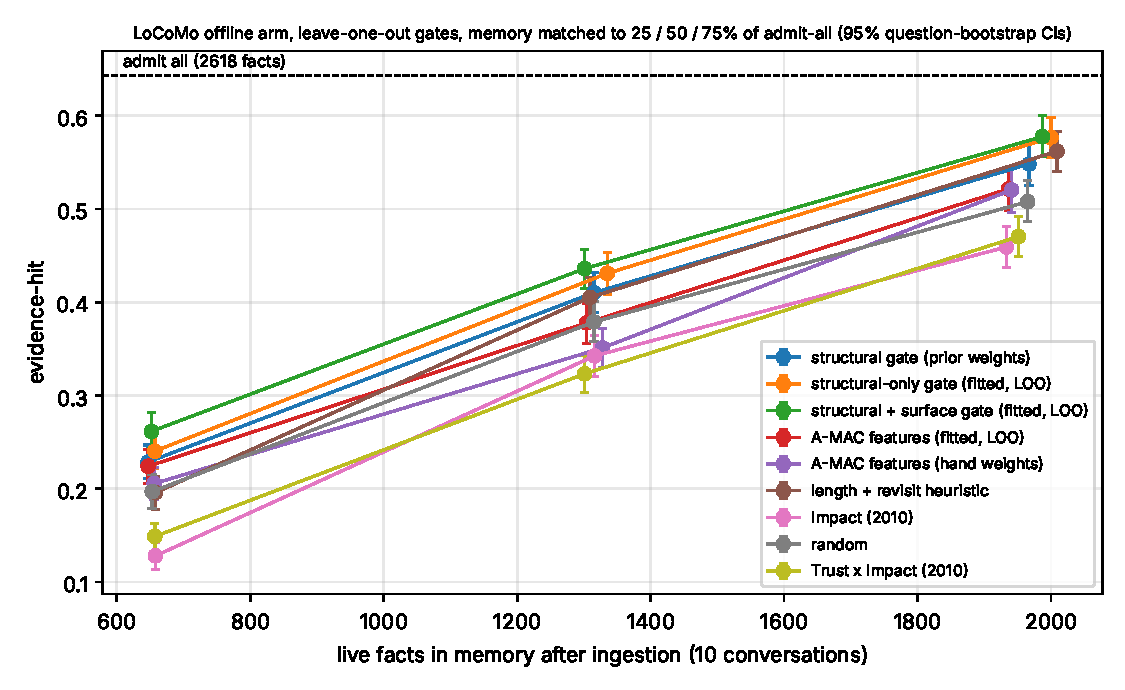
\includegraphics[width=0.78\linewidth]{../out/fig/budget_curve_hit.pdf}
  \caption{Evidence hit retained against memory size (fraction of admit-all's live facts), leave-one-conversation-out, all ten conversations as test units.}
  \label{fig:budget}
\end{figure}

\paragraph{Primary test.} Table~\ref{tab:perm} gives the exact sign-flip permutation test of the structural-only gate against every other policy at half size. The gate beats random (\permRandomMean{}, $p=\permRandomP$, Holm \permRandomHolm, \permRandomWins/10 conversations), the 2010 product (\permSivTenMean, Holm \permSivTenHolm, \permSivTenWins/10), Impact alone (\permImpactTenMean, Holm \permImpactTenHolm, \permImpactTenWins/10) and both A-MAC feature policies (\permAmacLiteMean{} and \permAmacFitMean, Holm \permAmacLiteHolm{} and \permAmacFitHolm). It does not reliably beat heat, the length-plus-revisit heuristic (\permHeatMean, $t$-interval [\permHeatCiLo, \permHeatCiHi], Holm \permHeatHolm, \permHeatWins/10), which is essentially turn length, the single strongest label correlate. Adding the six surface features to the structural gate changes nothing (\permGraphGateFullMean): the structural features and turn length carry overlapping information about what the annotators asked about. The hand-set prior gate is weaker than the fitted structural gate (\permGraphGateMean) and no better than heat.

\begin{table}[tp]
  \centering
  \caption{Exact sign-flip permutation over the ten conversations, structural-only gate minus each other policy, evidence hit at 50\% memory. Positive favours the gate. Holm over the eight comparisons of this table.}
  \label{tab:perm}
  \small
  \begin{tabular}{@{}lrrrrr@{}}
    \toprule
    Gate minus & Mean diff. & 95\% $t$-interval & $p_{\mathrm{perm}}$ & Holm & Conv.\ $>0$ \\
    \midrule
    random & \permRandomMean & [\permRandomCiLo, \permRandomCiHi] & \permRandomP & \permRandomHolm & \permRandomWins/10 \\
    SIV-2010 & \permSivTenMean & [\permSivTenCiLo, \permSivTenCiHi] & \permSivTenP & \permSivTenHolm & \permSivTenWins/10 \\
    impact-2010 & \permImpactTenMean & [\permImpactTenCiLo, \permImpactTenCiHi] & \permImpactTenP & \permImpactTenHolm & \permImpactTenWins/10 \\
    A-MAC-lite & \permAmacLiteMean & [\permAmacLiteCiLo, \permAmacLiteCiHi] & \permAmacLiteP & \permAmacLiteHolm & \permAmacLiteWins/10 \\
    A-MAC, fitted & \permAmacFitMean & [\permAmacFitCiLo, \permAmacFitCiHi] & \permAmacFitP & \permAmacFitHolm & \permAmacFitWins/10 \\
    heat & \permHeatMean & [\permHeatCiLo, \permHeatCiHi] & \permHeatP & \permHeatHolm & \permHeatWins/10 \\
    graph gate, prior & \permGraphGateMean & [\permGraphGateCiLo, \permGraphGateCiHi] & \permGraphGateP & \permGraphGateHolm & \permGraphGateWins/10 \\
    graph gate, full & \permGraphGateFullMean & [\permGraphGateFullCiLo, \permGraphGateFullCiHi] & \permGraphGateFullP & \permGraphGateFullHolm & \permGraphGateFullWins/10 \\
    \bottomrule
  \end{tabular}
\end{table}

\paragraph{Per category.} At half size the structural gate's evidence hit by category is single-hop \catLcSingleHopGraphGateStruct{} (random \catLcSingleHopRandom), multi-hop \catLcMultiHopGraphGateStruct{} (\catLcMultiHopRandom), temporal \catLcTemporalGraphGateStruct{} (\catLcTemporalRandom), open-domain \catLcOpenDomainGraphGateStruct{} (\catLcOpenDomainRandom) and adversarial \catLcAdversarialGraphGateStruct{} (\catLcAdversarialRandom); the admit-all ceiling is \catLcSingleHopAdmitAll, \catLcMultiHopAdmitAll, \catLcTemporalAdmitAll, \catLcOpenDomainAdmitAll{} and \catLcAdversarialAdmitAll. These are exploratory.

\subsection{Does the offline proxy predict answers? The online arm}
\label{sec:online}
Table~\ref{tab:online} answers the 1,986 questions with the fixed model on three memories: admit-all, the structural gate at half size and random at half size, in both verbalisation passes. Three things follow.

\begin{table}[tp]
  \centering
  \caption{Online arm: official LoCoMo token F1 and exact match from a fixed answerer, next to the offline evidence hit, for three memories. Pass 1 verbalises a fact as its observation sentence; pass 2 adds the observation date to every fact and the official temporal hint to temporal questions. Abstention is the share of answers equal to ``No information available''. Adversarial questions are scored by abstention, so a smaller memory scores higher on them.}
  \label{tab:online}
  \footnotesize
  \begin{tabular}{@{}llrrrrr@{}}
    \toprule
    Pass & Memory & Evidence hit & F1 & EM & Abstention & F1, temporal \\
    \midrule
    1 & admit-all & \hitOneAdmitAll & \foneOneAdmitAll & \emOneAdmitAll & \abstOneAdmitAll & \foneOneAdmitAllTemporal \\
    1 & structural gate, 50\% & \hitOneStruct & \foneOneStruct & \emOneStruct & \abstOneStruct & \foneOneStructTemporal \\
    1 & random, 50\% & \hitOneRandom & \foneOneRandom & \emOneRandom & \abstOneRandom & \foneOneRandomTemporal \\
    \midrule
    2 & admit-all & \hitTwoAdmitAll & \foneTwoAdmitAll & \emTwoAdmitAll & \abstTwoAdmitAll & \foneTwoAdmitAllTemporal \\
    2 & structural gate, 50\% & \hitTwoStruct & \foneTwoStruct & \emTwoStruct & \abstTwoStruct & \foneTwoStructTemporal \\
    2 & random, 50\% & \hitTwoRandom & \foneTwoRandom & \emTwoRandom & \abstTwoRandom & \foneTwoRandomTemporal \\
    \bottomrule
  \end{tabular}
\end{table}

\emph{The proxy carries signal.} Pooling the three memories and excluding the abstention-scored adversarial category, the mean F1 of a question whose gold-evidence fact was retrieved is \hitCondOneTwo{} against \hitCondZeroTwo{} when it was not (pass 2; \hitCondOneOne{} against \hitCondZeroOne{} in pass 1). The contrast is largest on single-hop questions (\hitCondDiffTwoSingleHop) and smallest on open-domain questions (\hitCondDiffTwoOpenDomain), whose gold answers are rarely a retrievable fact.

\emph{Undated facts cannot answer temporal questions.} In pass 1 the temporal F1 of the admit-all memory is \foneOneAdmitAllTemporal{} at an evidence hit of \hitOneAdmitAllTemporal: the gold fact is retrieved, but the fact store has stripped the date the question asks for. Appending the observation date and the official hint (pass 2) raises it to \foneTwoAdmitAllTemporal{} and the overall F1 from \foneOneAdmitAll{} to \foneTwoAdmitAll. Any evaluation of a fact-store memory on LoCoMo that omits one of the two under-reports temporal performance by this margin.

\emph{The proxy overstates the gate's benefit.} The structural gate's offline advantage over random at half size is \permRandomMean{} evidence hit ($p=\permRandomP$, \permRandomWins/10 conversations). The same two memories, answered, differ by \dFoneStructRandomOne{} F1 in pass 1 ($t$-interval [\ciFoneStructRandomLoOne, \ciFoneStructRandomHiOne], $p=\pFoneStructRandomOne$, \winsFoneStructRandomOne/10) and by \dFoneStructRandomTwo{} in pass 2 ([\ciFoneStructRandomLoTwo, \ciFoneStructRandomHiTwo], $p=\pFoneStructRandomTwo$, \winsFoneStructRandomTwo/10). The per-conversation differences in hit and in F1 agree in sign on \signAgreeTwo{} of ten conversations and are rank-correlated at \rhoDhitDfoneTwo{} (pass 2; \rhoDhitDfoneOne{} in pass 1), so the proxy orders conversations correctly while roughly halving the effect, from a result that is clear at $k=10$ to one at the edge of significance. Retrieving a gold fact is necessary for answering but not sufficient: the answerer still has to extract the answer from a one-sentence fact, and a memory that holds half the facts drives abstention to \abstTwoStruct{} of questions. The size of the effect that an offline sweep reports should be read as an upper bound on what a user would see, and dated facts with the official hint (pass 2) are the verbalisation under which the proxy tracks answers best.

\subsection{H1: the Mem0 gate as the LLM baseline}
\label{sec:h1}
The verbatim Mem0 gate, run over all \memzNconv{} conversations with the same model, returns \memzAdd{} \textsc{add}, \memzUpdate{} \textsc{update}, \memzDelete{} \textsc{delete} and \memzNone{} \textsc{none} events over \memzCalls{} calls (\memzParseFail{} unparseable responses) and admits a share \memzAdmitRate{} of candidate turns (per conversation \memzAdmitRateMin--\memzAdmitRateMax), a memory of \memzLive{} live facts, a fraction \memzFracOfAdmitAll{} of admit-all's. Its evidence hit is \memzHit{} against admit-all's \hitLcAdmitAll. The cost is \memzCallsPerK{} calls and \memzTokensPerK{} tokens per thousand candidate facts (one call per candidate turn). On distilled observations, which already are the ``facts'' a Mem0 extraction call would produce, the gate finds almost nothing to reject: the \textsc{update} and \textsc{delete} paths that make it a gate in the first place are reached \memzUpdate{} and \memzDelete{} times in \nObsSentences{} sentences, and \textsc{none} is returned for old memories, not for candidates. The pre-registered non-inferiority contrast is therefore run at the Mem0 gate's own realised size: the structural gate matched to that size reaches an evidence hit of \hitStructAtMemz{} and an F1 of \foneStructAtMemz{} against the Mem0 memory's \foneMemz{} (difference \hOneDiffFone{} F1 points, $t$-interval [\hOneCiLo, \hOneCiHi], inside the pre-registered 2.0-point margin; random at that size \foneRandomAtMemz). H1 therefore holds on LoCoMo (its LongMemEval-S half, 2.0 accuracy points, is untested), but trivially: at a memory size the LLM gate cannot be asked to change, the question ``is the LLM-free gate within two points'' is answered by construction, and the substantive finding of this arm is that the LLM gate spends one call per candidate turn (\memzCallsPerK{} per thousand candidate facts) to admit \memzAdmitRate{} of those turns. Whether Mem0's gate is selective on raw turns rather than on pre-distilled observations is a question for the LLM-extraction arm.

\subsection{A second dataset: LongMemEval-S}
\label{sec:lme}
LongMemEval-S gives each of \lmeNq{} questions its own haystack of 38 to 62 sessions, so each question is an independent memory and the question is the unit of inference. Candidates come from a \emph{heuristic extractor} used only on this dataset: each sentence of a user or assistant turn that opens in the first person (``I'', ``I'm'', ``I've'', ``My'', ``We'', ``Our'') goes through the dependency rule of Section~\ref{sec:design} with the turn's speaker as subject, at tier extractor-inferred (confidence 0.8), and the hub set is \{user, assistant\} (a placeholder for the LLM-extraction arm; assistant turns yield a candidate only when a sentence is first-person, which the answer-bearing assistant turns of the single-session-assistant type rarely are, so that type is near zero for every policy); admit-all holds \lmeLiveAdmitAll{} live facts over the \lmeNq{} memories, about 335 per question-memory against LoCoMo's 262 per conversation-memory (\liveLcAdmitAll{} over ten), and only one candidate in a hundred is gold evidence. Memory is matched by bisection to 50\% of admit-all per question. Two gates are run: the hand-set prior weights of Section~\ref{sec:measures} (\code{graph\_gate}) with no fitting, and the seven structural features fitted by five-fold cross-fitting over questions (each fold fitted on the admit-all candidate turns of the other 400 questions; grouped CV AUC \lmeCvAucMin--\lmeCvAucMax; the largest weights are the 2010 impact term, \lmeWImpactMin{} to \lmeWImpactMax{} across folds, and pattern novelty, \lmeWNoveltyMin{} to \lmeWNoveltyMax). No LoCoMo weights are used.

\begin{table}[tp]
  \centering
  \caption{LongMemEval-S, \lmeNq{} questions, memory matched to 50\% of admit-all per question. Evidence hit, evidence fraction and MRR of the retrieved set; paired per-question sign-flip permutation tests on the \lmeKHitFitRandom{} questions with gold evidence, fitted gate minus each other policy, Holm over the three.}
  \label{tab:lme}
  \footnotesize
      \begin{tabular}{@{}lrrrr@{}}
    \toprule
    Policy & Hit & Frac & MRR & Live \\
    \midrule
    admit-all & \lmeHitAdmitAll & \lmeFracAdmitAll & \lmeMrrAdmitAll & \lmeLiveAdmitAll \\
    graph gate, structural, cross-fitted & \textbf{\lmeHitFit} & \lmeFracFit & \lmeMrrFit & \lmeLiveFit \\
    graph gate, prior & \lmeHitPrior & \lmeFracPrior & \lmeMrrPrior & \lmeLivePrior \\
    random & \lmeHitRandom & \lmeFracRandom & \lmeMrrRandom & \lmeLiveRandom \\
    heat & \lmeHitHeat & \lmeFracHeat & \lmeMrrHeat & \lmeLiveHeat \\
    \bottomrule
  \end{tabular}\par\medskip
  \begin{tabular}{@{}lrrrrr@{}}
    \toprule
    Fitted gate minus & Hit difference & 95\% $t$-interval & $p_{\mathrm{perm}}$ & Holm & Wins/losses \\
    \midrule
    graph gate, prior & \lmeDHitFitPrior & [\lmeCiLoHitFitPrior, \lmeCiHiHitFitPrior] & \lmePHitFitPrior & \lmeHolmHitFitPrior & \lmeWinsHitFitPrior/\lmeLossesHitFitPrior \\
    random & \lmeDHitFitRandom & [\lmeCiLoHitFitRandom, \lmeCiHiHitFitRandom] & \lmePHitFitRandom & \lmeHolmHitFitRandom & \lmeWinsHitFitRandom/\lmeLossesHitFitRandom \\
    heat & \lmeDHitFitHeat & [\lmeCiLoHitFitHeat, \lmeCiHiHitFitHeat] & \lmePHitFitHeat & \lmeHolmHitFitHeat & \lmeWinsHitFitHeat/\lmeLossesHitFitHeat \\
    \bottomrule
  \end{tabular}
\end{table}

Three things follow (Table~\ref{tab:lme}), two of them different from LoCoMo. The turn-length heuristic is \lmeDHitRandomHeat{} \emph{below} random ($p=\lmePHitRandomHeat$): in a fifty-session haystack the long user turns are rarely the evidence, so its parity with the gate on LoCoMo was a statement about LoCoMo's annotators, not about the gate. The hand-set prior weights do not transfer: the unfitted gate is level with random on hit (\lmeDHitPriorRandom, $p=\lmePHitPriorRandom$) and only marginally ahead on rank (MRR \lmeDMrrPriorRandom, $p=\lmePMrrPriorRandom$, $t$-interval [\lmeCiLoMrrPriorRandom, \lmeCiHiMrrPriorRandom]), so the weights must be fitted per dataset, a deviation from the single held-out fit the pre-registration described. Fitted on the dataset itself with no question in its own fold's fit (filler sessions shared between haystacks do recur across folds, always with label 0), the structural-only gate retains \lmeDHitFitRandom{} more gold evidence than random at the same memory size (Holm $p=\lmeHolmHitFitRandom$, \lmeWinsHitFitRandom{} wins to \lmeLossesHitFitRandom{} losses) and \lmeDMrrFitRandom{} more MRR ($p<0.001$); per type it leads most on multi-session (\lmeHitFitMultiSession{} vs \lmeHitRandomMultiSession) and knowledge-update (\lmeHitFitKnowledgeUpdate{} vs \lmeHitRandomKnowledgeUpdate) questions. The matched-size claim therefore rests on two datasets with two independent units of inference, and the fitted weights say that on a long haystack the ``attached to what memory already holds'' signal, useless on LoCoMo, is the one that carries information. The offline proxy has not been validated against answers on this dataset, and the extractor still produces no entity-to-entity edges (non-hub edge share 0.000 in the admit-all run); both are stated as limits in Section~\ref{sec:threats}.

\subsection{H3, exploratory: are facts about new entities worth more?}
\label{sec:h3}
The 2010 prior says disconnected new knowledge is worth less than knowledge attached to known vertices. Table~\ref{tab:h3} contrasts candidate turns whose non-hub vertices are all new ($\Anc=0$) with turns whose non-hub vertices are all known ($\Anc=1$) by the share that are gold evidence turns of a question of the category. The all-new turns are evidence more often in every category (\hThreeDiffAll{} overall, intervals \hThreeNewCiAll{} against \hThreeKnownCiAll); the direction is the inversion H3 predicts, on every LoCoMo category, but the measure is evidence-label rate rather than the pre-registered per-fact answer-value delta, and the two groups differ in size by a factor of four, so we report it as exploratory; the pre-registered confirmation rule, inversion on the two single-session LongMemEval types, has not been evaluated.

\begin{table}[tp]
  \centering
  \caption{Exploratory H3 on LoCoMo: share of candidate turns that are gold evidence of a question in the category, for turns whose non-hub vertices are all new ($\Anc=0$) against all known ($\Anc=1$), with Wilson 95\% intervals. Turns with no non-hub vertex are excluded.}
  \label{tab:h3}
  \small
  \begin{tabular}{@{}lrrrrr@{}}
    \toprule
    Category & $\Anc=0$ (new) & 95\% CI & $\Anc=1$ (known) & 95\% CI & Difference \\
    \midrule
    single-hop & \hThreeNewSingleHop & \hThreeNewCiSingleHop & \hThreeKnownSingleHop & \hThreeKnownCiSingleHop & \hThreeDiffSingleHop \\
    multi-hop & \hThreeNewMultiHop & \hThreeNewCiMultiHop & \hThreeKnownMultiHop & \hThreeKnownCiMultiHop & \hThreeDiffMultiHop \\
    temporal & \hThreeNewTemporal & \hThreeNewCiTemporal & \hThreeKnownTemporal & \hThreeKnownCiTemporal & \hThreeDiffTemporal \\
    open-domain & \hThreeNewOpenDomain & \hThreeNewCiOpenDomain & \hThreeKnownOpenDomain & \hThreeKnownCiOpenDomain & \hThreeDiffOpenDomain \\
    adversarial & \hThreeNewAdversarial & \hThreeNewCiAdversarial & \hThreeKnownAdversarial & \hThreeKnownCiAdversarial & \hThreeDiffAdversarial \\
    \midrule
    any question & \hThreeNewAll & \hThreeNewCiAll & \hThreeKnownAll & \hThreeKnownCiAll & \hThreeDiffAll \\
    \multicolumn{6}{@{}l}{$n=\hThreeNnewAll$ turns with $\Anc=0$ and $n=\hThreeNknownAll$ with $\Anc=1$.} \\
    \bottomrule
  \end{tabular}
\end{table}

\subsection{H4: poisoning and the provenance tier}
\label{sec:h4}
Table~\ref{tab:poison} reports the poisoning arm at a 10\% per-dialogue-turn injection rate (just over a quarter of the candidate stream) and 50\% memory over \poisN{} injected facts. When the poison carries the same tier confidence as real candidates (\emph{sourceless}), both graph gates, prior and structural-only, admit \emph{more} of it than random (\poisAdmitGraphGateStructTenSrc{} and \poisAdmitGraphGateTenSrc{} against \poisAdmitRandomTenSrc), and the tier multiplier has, by construction, no effect. Fabricated facts about hub-adjacent entities with real-vocabulary predicates are novel and anchored in exactly the way the gate rewards. When the poison carries a lower tier and the score is multiplied by tier confidence, poison admission falls to \poisAdmitGraphGateStructTenTier{} and \poisAdmitGraphGateTenTier{} (random with the multiplier \poisAdmitRandomTenTier), and evidence hit rises, from 0.300 to 0.403 for the structural-only gate and from 0.294 to 0.378 for the prior gate (overall hit in the run summaries \code{merged\_poison\_*}), because poison stops displacing real facts within the same budget. Nearly every question still retrieves at least one injected fact (\poisRetrievedShareGraphGateStructTenTier{} of questions under the best condition), so the retrieval-level harm of this injection rate needs the online arm. The statement the arm supports is that structural novelty is blind to truth and that provenance weighting, not structure, is the defence; the sourceless condition is the honest ceiling on what an attacker who can forge the provenance route achieves, as Fei et al.'s accumulability criterion predicts for a reallocatable retrieval selector, here carried over to an admission score~\cite{fei2026selection}.

\begin{table}[tp]
  \centering
  \caption{Poisoning arm, one fabricated fact per dialogue turn with probability 10\% (just over a quarter of the candidate stream), memory 50\%, \poisN{} injected facts paired across policies. Sourceless: poison tier confidence equals the real candidates'. Lower: poison tier 0.4 against 0.6. $\times$tier: the policy score is multiplied by mean tier confidence. ``Questions with poison'' is the share of questions whose retrieved set holds at least one injected fact.}
  \label{tab:poison}
  \small
  \begin{tabular}{@{}llrr@{}}
    \toprule
    Condition & Policy & Poison admitted & Questions with poison \\
    \midrule
    sourceless & random & \poisAdmitRandomTenSrc & \poisRetrievedShareRandomTenSrc \\
    sourceless & graph gate, prior & \poisAdmitGraphGateTenSrc & \poisRetrievedShareGraphGateTenSrc \\
    sourceless & graph gate, structural & \poisAdmitGraphGateStructTenSrc & \poisRetrievedShareGraphGateStructTenSrc \\
    \midrule
    lower $\times$tier & random & \poisAdmitRandomTenTier & \poisRetrievedShareRandomTenTier \\
    lower $\times$tier & graph gate, prior & \poisAdmitGraphGateTenTier & \poisRetrievedShareGraphGateTenTier \\
    lower $\times$tier & graph gate, structural & \poisAdmitGraphGateStructTenTier & \poisRetrievedShareGraphGateStructTenTier \\
    \bottomrule
  \end{tabular}
\end{table}

\subsection{Why the graph has no topology, and where it could}
\label{sec:shape}
The zero share of entity-to-entity edges is not an extractor artefact. Parsing all \nObsSentences{} observation sentences, the grammatical subject of the main verb is a speaker's name in \obsSpeakerSubjShare{} of sentences, a speaker's possessive (``Melanie's kids'') in \obsPossSubjShare, unparsable in \obsParseFailShare, and any other entity or common noun in \obsNonSpeakerSubjShare. The benchmark's own observations are written as ``Caroline did $X$''. We simulated three LLM-free rules on top of the current extraction: keeping a relation noun's appositive name as subject (``Caroline's husband John works at Dell'' $\to$ (John, works\_at, Dell)) yields \emph{zero} edges in the corpus; keeping a non-speaker nominal subject yields at most \ruleBedgesMax{} edges per conversation, of poor quality; linking the primary object to every other named entity of the sentence (``co-mentioned with'') yields \ruleCedgesMin--\ruleCedgesMax{} edges per conversation and would raise the non-hub edge share to between 2\% and 20\% of live edges, but the edge is not a relation and would turn anchoring into a within-sentence co-occurrence count. Nor would an LLM extractor on the raw turns help on this dataset: \rawTurnsOneNE{} of turns mention a third-party named entity and \rawTurnsTwoNE{} mention two, the precondition for an entity-to-entity fact. On LongMemEval-S, by contrast (spaCy NER over the user turns of the first 40 questions; the LoCoMo figures are over the raw turns of the first three conversations), \lmeTurnsOneNE{} of user turns mention a third-party entity and \lmeTurnsTwoNE{} mention two, fifteen times LoCoMo's density. That, and the knowledge-update question type, is where the realised-change hypothesis H2, the consolidation step and any genuinely structural claim have to be tested; the graph-shape precondition table of Section~\ref{sec:degeneracy} is printed before every such run.

\subsection{Cost}
Admit-all and the nine LLM-free admission policies make no write-path model call. The Mem0 gate makes \memzCallsPerK{} calls and \memzTokensPerK{} tokens per thousand candidate facts. The online arm of this paper (two passes over three memories, the Mem0 gate and its matched comparison) took \haikuCalls{} model calls, \haikuInTokens{}M input and \haikuOutTokens{}M output tokens, about \$\haikuCostUsd{} at list price, with thinking disabled; with thinking enabled, as the model runs by default, 15\% of gate calls were truncated at the 256-token budget of the 19 October smoke test, which is why the adapter disables it.

% =====================================================================
\section{Threats to validity}
\label{sec:threats}

\paragraph{Construct.} Evidence hit is a proxy, and Section~\ref{sec:online} measures by how much it overstates: a policy effect of \permRandomMean{} in hit became \dFoneStructRandomTwo{} in F1 ($p=\pFoneStructRandomTwo$). The admission label used to fit the gate (``the source turn is a gold evidence turn'') is relevance to the benchmark's questions, not value in general; leakage is prevented by leave-one-conversation-out fitting, but a gate fitted this way is tuned to the benchmark's question distribution, and turn length is its best single predictor, which says as much about how annotators choose questions as about memory. The 2010 measures were designed for document-sized targets against an encyclopaedic context; we test them at a granularity their authors did not intend, which is the point of the degeneracy analysis, but it means the result is about the formulation at fact granularity.

\paragraph{Internal.} Entity-resolution errors create spurious degree, GAM's ``lexical noise'' objection~\cite{gam2026}; the hand check of Section~\ref{sec:design} is \extHandCheckN{} triples read by a single annotator and the 200-mention entity-resolution precision sample is owed; on LongMemEval-S the heuristic extractor has had no hand check at all. The oracle arm's candidates are gpt-3.5-turbo observations that cover 76\% of gold evidence turns and pre-select which turns yield candidates at all; admit-all's ceiling of \hitLcAdmitAll{} is a property of that coverage. The graph is two stars, so anchoring, impact and $\Tedge$ are near-constant and their non-zero values measure recurrence (Section~\ref{sec:shape}). Consolidation never fires, so the predicted/actual distinction is void in this arm and H2 is untested rather than null. The gate's weights are fitted on features computed along an admit-all trajectory but applied to the smaller graph the gate itself builds. The answerer is one model with thinking disabled; its abstention behaviour (\abstTwoAdmitAll{} on the full memory) sets the F1 scale, and the adversarial category rewards abstention, so smaller memories score higher there. Random admission uses one seed. On LongMemEval-S the extractor is a first-person heuristic with no hand check, about a third of its candidate turns are assistant turns, and the fitted weights put most mass on the 2010 impact term, whose variation in a star-shaped graph measures recurrence of objects around the two hubs rather than topology.

\paragraph{External.} Two English benchmarks, both dyadic; speakers (or the user) as hubs is a property of dyadic chat, and the LongMemEval-S arm is offline only. The poisoner is synthetic and non-adaptive; the pre-registered 0/2/10\% grid and QA harm are not run. The Mem0 gate was run on pre-distilled observations, where it is not selective; its behaviour on raw turns is untested here.

\paragraph{Statistical.} Ten conversations is the honest unit on LoCoMo and the smallest attainable permutation $p$ is 0.002; on LongMemEval-S the unit is the question, the sign-flip test over \lmeKHitFitRandom{} questions samples 20,000 sign assignments rather than enumerating them, and filler sessions shared between haystacks put identical label-0 candidates in a fold's fit and its held-out questions; the Holm families are those of each table, not the pre-registered four-hypothesis family. The question-level bootstrap is anti-conservative and reported as secondary. Matched size says nothing about what a policy does at another size; the curves of Figure~\ref{fig:budget} are reported for that.

\paragraph{Framing.} ``LLM-free'' describes the gate, not the write path: the LoCoMo oracle arm consumes model-generated observations, so only the LongMemEval-S arm, whose extractor reads raw user turns, is model-free from the turn text onward. The precise claim is zero model calls at the gate, given an extractor.

% =====================================================================
\section{Conclusion}
\label{sec:conclusion}
We took a 2010 measure of the value of information to a graph-shaped world view, showed where it breaks when the world view is an agent's memory and the information is a single conversational fact, repaired it without adding a model call, and tested it under a pre-registered protocol with everything but the admission policy held fixed. The verdicts are: the 2010 trust-times-impact product and Impact alone are the two worst admission policies at every budget, below random throughout, for arithmetic reasons that any fact-granular use of them will share; the repaired, LLM-free gate beats random, the 2010 measures and lexical features at matched size on LoCoMo but is no better than turn length there, and its offline advantage shrinks by about half, to the edge of significance over ten conversations, when the questions are actually answered; on LongMemEval-S the same gate, cross-fitted over \lmeNq{} questions and tested on the \lmeKHitFitRandom{} with gold evidence, beats random by \lmeDHitFitRandom{} while turn length falls below random, so the advantage is real but its weights are dataset-specific; the verbatim Mem0 gate does not gate on distilled observations, so the pre-registered non-inferiority question becomes a cost question on this benchmark; facts about new entities are, exploratorily, gold evidence more often than facts about known ones, against the 2010 prior; and structural novelty admits more poison than random unless provenance is weighted. The realised-change hypothesis and every genuinely topological claim move to LongMemEval-S with an LLM extractor, where the data has the structure that LoCoMo lacks. The measures remain al-Saffar and Heileman's; what is new is the evidence, including the negative parts.

\section*{Supplementary Material Statement}
Code (\code{paper2/}), the frozen pre-registration with its implementation log and deviations, the verbatim Mem0 prompt module with attribution, run artefacts (\code{paper2/out/}) and the number files behind every table (\code{paper2/paper/numbers.tex}, \code{numbers\_online.tex}, \code{numbers\_lme.tex}) are released at \ifanon an anonymised mirror, \todo{anonymised repository URL}, with the public repository to follow acceptance\else \url{https://github.com/zubertaj123/context-graph-research}\fi{} (a Zenodo DOI for the tagged release will be added in the next version) under MIT (code), CC BY 4.0 (paper, documents and run artefacts). LoCoMo is used under its own licence; the Mem0 prompt is Apache-2.0; no proprietary data is used.

\ifceur\begin{acknowledgments}\else\ifllncs\begin{credits}\subsubsection{\ackname}\else\section*{Acknowledgements and attribution}\fi\fi
Trust, impact and the two semantic information values are the work of Sinan al-Saffar and Gregory Heileman~\cite{alsaffar2008impact,alsaffar2008valuation,alsaffar2010siv}; the extant ontology is al-Saffar, Joslyn and Chappell's and the motif information gain is Joslyn, al-Saffar, Haglin and Holder's~\cite{alsaffar2011extant,joslyn2011motifs}. This paper implements and evaluates those measures; it does not claim them. The author has not been in contact with Dr.\ al-Saffar; the attribution above is the acknowledgement, and if Dr.\ al-Saffar can be reached, an offer of acknowledgement or co-authorship will be made, as the pre-registration commits to, before any venue submission.
\ifceur\end{acknowledgments}\else\ifllncs\subsubsection{\discintname} The author has no competing interests to declare that are relevant to the content of this article.\end{credits}\fi\fi

\section*{Declaration on Generative AI}
During the preparation of this work the author used a large-language-model coding assistant (Claude, Anthropic) to draft code, the LaTeX, the related-work notes and parts of the prose from the pre-registration document and the run logs, and to run the experiments. Claude Haiku 5.5 is also the fixed answerer of the online arm and the model behind the Mem0 gate baseline, as described in Section~\ref{sec:design}. The author reviewed and edited the content and takes full responsibility for the publication's content.

\ifceur
  \bibliographystyle{unsrt}
\else
  \IfFileExists{splncs04.bst}{\bibliographystyle{splncs04}}{\bibliographystyle{unsrt}}
\fi
\bibliography{refs}
\end{document}
